\section{Distributional RL}

\subsection{Идея Distributional подхода}

\needspace{7\baselineskip}
\begin{wrapfigure}{r}{0.25\textwidth}
\vspace{-0.3cm}
\centering
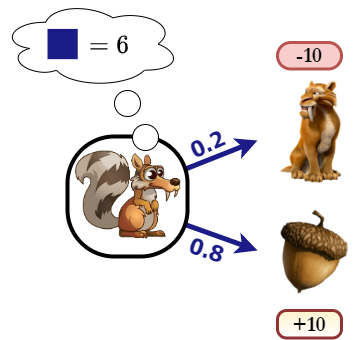
\includegraphics[width=0.25\textwidth]{Images/DistributionalRL1.png}
\vspace{-0.6cm}
\end{wrapfigure}

Задача RL такова, что в среде содержится в том числе неподконтрольная агенту стохастика: \emph{алеаторическая неопределённость} (aleatoric uncertainty)\footnote{которую не стоит путать с \emph{эпистемической неопределённостью} (epistemic uncertainty), или байесовской неопределённостью, связанной с нашим субъективным незнанием о том, как устроена, например, функция переходов и награды на самом деле, связанной с нашим осознанием неточности прогнозов.}. Агент, предсказывающий, что он получит в будущем в среднем суммарную награду 6, на самом деле может получить, например, только -10 или 10, просто последний исход случится с вероятностью 0.8, а первый --- 0.2. Помимо прочего, это означает, что часто агенту приходится рисковать: например, теоретически возможна ситуация, когда агент с малой вероятностью получает гигантскую награду, и тогда оптимальный агент на практике будет постоянно получать, например, какой-то штраф, компенсирующийся редко выпадающими мегаудачами. Вся эта информация заложена в распределении награды $R(\Traj)$ \eqref{return} как случайной величины.

\needspace{7\baselineskip}
\begin{wrapfigure}{l}{0.3\textwidth}
\vspace{-0.3cm}
\centering
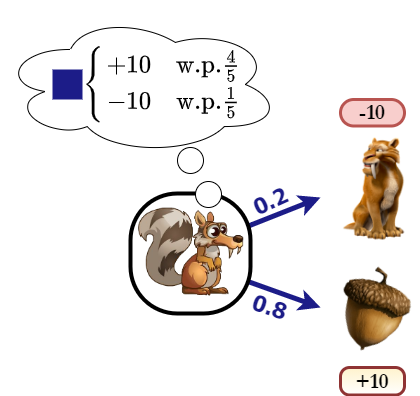
\includegraphics[width=0.3\textwidth]{Images/DistributionalRL2.png}
\vspace{-0.3cm}
\end{wrapfigure}

В Distributional-подходе предлагается учить не среднее будущей награды, а всё распределение будущей награды как случайной величины. Складывается эта неопределённость как из подконтрольной агенту стохастики --- его собственных будущих выборов действий --- так и неподконтрольной, переходов (и награды, если рассматривается формализм со случайной функцией награды). Среднее есть лишь одна из статистик этого распределения. 

Здесь стоит заранее оговориться о противоречиях, связанной с этой идеей. Обсуждение этой темы в первую очередь мотивировано эмпирическим превосходством Distributional-подхода по сравнению с алгоритмами, учащими только среднее, однако с теоретической точки зрения ясного обоснования этого эффекта нет. Даже наоборот: мы далее встретим теоретические результаты, показывающие эквивалентность Distributional-алгоритмов с обычными в рамках табличного сеттинга. 

Одно гипотетическое объяснение преимущества distributional-подхода в нейросетевом сеттинге, когда будущая награда предсказывается сложной параметрической моделью, может быть следующая: обучая модель предсказывать не только среднее награды, но и другие величины (другие статистики), сильно связанные по смыслу со средней наградой, в модель отправляются более информативные градиенты. Например, если с вероятностью 0.01 во входном изображении появляется грибочек, намекающий на приближение вкусного +100, обновление среднего будет, абстрактно говоря, проходить с учётом малой вероятности явления; когда обучение 1\%-го квантиля наоборот крайне интересуется именно хвостом распределения и поможет быстрее выучить, например, фильтр для детекции грибочка в первых свёрточных слоях, который, в свою очередь, ускорит и более точное вычисление среднего, для которого распознавание грибочка на самом деле было существенным.

\begin{remark}
Ещё одним способом придумать для модели целевую переменную, предсказание которой сильно связано со средней наградой, является использование нескольких дискаунт-факторов $0 \HM< \gamma_1 \HM< \gamma_2 \HM< \dots \HM< \gamma_G \HM< \gamma$, где $\gamma$ --- коэффициент, для которого решается задача. Иначе говоря, нейросетевая модель выдаёт для каждой пары состояние-действие не одно, а $G+1$ число, соответствующее $Q$-функции для соответствующего коэффициента дисконтирования:
$$Q^\pi(s, a, g) \coloneqq \E_{\Traj \mid s_0 = s, a_0 = a} \sum_{t \ge 0} \gamma_g^t r_t, \quad g \in \{1 \dots G \}$$
Иными словами, мы дополнительно учим, какую награду мы получим в самое ближайшее время, более близкое, чем реальный рассматриваемый горизонт. Эти дополнительные величины самой стратегией использоваться не будут (взаимодействие со средой использует только значения $Q$ для настоящего коэффициента $\gamma$), однако их обучение поможет <<ускорить>> обучение для настоящей $Q$ с самым большим горизонтом. Мы вернёмся к обобщению этой идеи, когда будем обсуждать multi-task RL в разделе \ref{sec:multitask}.
\end{remark}

\subsection{Z-функция}

\begin{definition} 
Для данного MDP \emph{оценочной функцией в distributional форме} (distributional state-action value function) для стратегии $\pi$ называется случайная величина, обусловленная на пару состояние-действие $s, a$ и определяющаяся как reward-to-go для такого старта:
$$\Z^\pi(s, a) \cdfcoloneqq R(\Traj), \qquad \Traj \sim \pi \mathrel{\Big|} \, s_0 = s, a_0 = a $$
\end{definition}

Здесь читателю предлагается заварить себе кофе на том факте, что введённая так называемая Z-функция\footnote{слово <<функция>> здесь, конечно, не очень удачно, однако автор данного текста не справился с нахождением альтернатив. <<Величина>> ещё можно было бы.} является для каждой пары $s, a$ случайной величиной. Во-первых, это скалярная случайная величина, соответственно, она задаётся некоторым распределением на $\R$, во-вторых, как и для любой случайной величины, существенно, на что она обуславливается. Запись $\Z^\pi(s, a)$ предполагает, что мы сидим в состоянии $s$ и выполнили действие $a$, после чего <<бросаем кости>> для сэмплирования случайной величины; нас, вообще говоря, будет интересовать её \emph{функция распределения} (cumulative distribution function, c.~d.~f.):
$$F_{\Z^\pi(s, a)}(x) \coloneqq \Prob (\Z^\pi(s, a) \le x)$$
Нам будет удобнее работать с ними, а не с плотностями, поскольку зачастую распределение $\Z^\pi(s, a)$ --- дискретное или вообще \emph{вырожденное} (принимающее с вероятностью 1 только какое-то одно значение). Таким образом, пространство всевозможных Z-функций имеет такой вид:
\begin{equation}\label{Zfunctionspace}
\Z^\pi(s, a) \in \St \times \A \to \Prob (\R),
\end{equation}
где $\Prob (\R)$ --- пространство скалярных случайных величин. 

Надпись c.d.f. над равенством здесь и далее означает, что слева и справа стоят случайные величины. Очень важно, что случайные величины справа и слева в подобных равенствах обусловлены на одну и ту же информацию: справа, как и слева, стоит случайная величина, обусловленная на $s, a$. Случайная величина здесь задана процессом генерации: сначала генерируется случайная траектория $\Traj$ при заданных $s_0 \HM= s, a_0 \HM= a$ (это по определению MDP эквивалентно последовательному сэмплированию $s_1, a_1, s_2 \dots$), затем от этой случайной величины считается детерминированная функция $R(\Traj)$. Запись $\cdfcoloneqq$ означает, что $\Z^\pi(s, a)$ имеет в точности то же распределение, что и случайная величина, генерируемая процессом, описанном справа.

По определению:

\begin{proposition}
\begin{equation}\label{QZ}
Q^\pi(s, a) = \E \Z^\pi(s, a)
\end{equation}
\end{proposition}

\begin{proposition}
В терминальных состояниях для всех действий $\Z^{\pi}(s, a)$ есть вырожденная случайная величина, с вероятностью 1 принимающая значение ноль.
\end{proposition}

\needspace{16\baselineskip}
\begin{exampleBox}[label=ex:zfunction]{}
Посчитаем Z-функцию для MDP и стратегии $\pi$ с рисунка, $\gamma \HM= 0.8$.

\begin{wrapfigure}{r}{0.45\textwidth}
\vspace{-0.4cm}
\centering
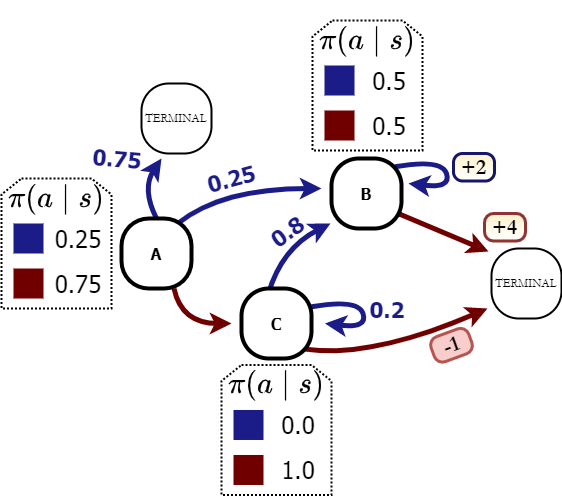
\includegraphics[width=0.45\textwidth]{Images/Value.png}
\vspace{-0.4cm}
\end{wrapfigure}

Начнём с состояния B: если агент выбирает действие \colorsquare{ChadRed}, то он получает +4, и эпизод заканчивается. Значит, $\Z^{\pi}(s \HM= B, \colorsquare{ChadRed})$ всегда принимает значение 4.

Что произойдёт, если он выберет \colorsquare{ChadBlue}? Агент точно получит +2 и вернётся в состояние B. Вся дальнейшая награда будет дисконтирована на $\gamma \HM= 0.8$. После этого начинается первая стохастика: агент снова будет выбирать действие! С вероятностью 0.5 он выберет \colorsquare{ChadRed} и получит итоговый reward-to-go $2 \HM+ \gamma \cdot 4 \HM= 5.2$ за эпизод. Вот мы нашли часть нашей Z-функции для $s \HM= B$, $a \HM= \colorsquare{ChadBlue}$: с вероятностью 0.5 исход будет 5.2. Ищем, что соответствует оставшейся вероятностной массе 0.5: мы выберем снова \colorsquare{ChadBlue}, получим уже суммарно $2 \HM+ \gamma \cdot 2 \HM= 3.6$, снова вернёмся в B, снова случится дисконтирование и снова за нами будет выбор. Мы можем найти, что соответствует ещё 0.25 нашей вероятностной массы: $2 \HM+ \gamma \cdot 2 + \gamma^2 \cdot 4 \HM= 6.16$. Дальше в этом распределении будет ещё исход с вероятностью $\frac{1}{8}$, затем $\frac{1}{16}$ и так далее: $\Z^{\pi}(s \HM= B, \colorsquare{ChadBlue})$ есть распределение со счётным множеством исходов!

Очевидно, что $\Z^{\pi}(s \HM= A, \text{\colorsquare{ChadRed}})$ и $\Z^{\pi}(s \HM= C, \text{\colorsquare{ChadRed}})$ тоже будут вырожденными: reward-to-go для таких стартов однозначно определён и равен -0.8 и -1 соответственно. 

$\Z^{\pi}(s \HM= A, \text{\colorsquare{ChadBlue}})$ содержит компоненту <<с вероятностью 0.75 мы попадём в терминальное состояние и получим 0>>. Оставшиеся 0.25 соответствуют попаданию в B и распределяются пополам между выбором следующего действия \colorsquare{ChadRed} (соответствует награде 3.2) и \colorsquare{ChadBlue} (тогда начнётся та же цепочка исходов, домноженных на $\gamma \HM= 0.8$, что и для $\Z^{\pi}(s \HM= B, \colorsquare{ChadBlue})$). Аналогично можно расписать $\Z^{\pi}(s \HM= C, \text{\colorsquare{ChadBlue}})$; как видно, такая <<оценочная функция>> содержит в себе намного больше информации о будущих наградах.
\end{exampleBox}

\subsection{Distributional-форма уравнения Беллмана}

Заметим, что в доказательстве уравнений Беллмана, например, \eqref{VV}, мы ссылаемся на то, что для reward-to-go любых траекторий верно рекурсивное соотношение. После этого мы берём по траекториям мат.ожидание слева и справа, получая традиционное уравнение Беллмана. Ясно, что мы могли бы вместо среднего взять любую другую статистику от случайной величины (дисперсию, медианы, другие квантили...), а, вообще говоря, верно совпадение левой и правой части по распределению. Иначе говоря, мы зачёркиваем символ мат.ожидания из уравнения Беллмана для получения более общего утверждения.

\begin{theorem}[Уравнение Беллмана в Distributional-форме]\,
\begin{equation}\label{ZZ}
 \Z^\pi(s, a) \cdfeq r(s, a) + \gamma \Z^\pi(s', a'), \quad s' \sim p(s' \mid s, a), a' \sim \pi(a' \mid s') 
\end{equation}
\begin{proof}
Следует из тождества $R(\Traj) = r + \gamma R(\Traj_{1:})$ для любых траекторий $\Traj$.
\end{proof}
\end{theorem}

Читатель подозревается в недоумении от происходящего; остановимся на этом уравнении и обсудим, что тут написано. Во-первых, необходимо пояснить, что данное уравнение есть переформулировка (другая нотация) используемых определений. Reward-to-go $R(\Traj)$ --- детерминированная функция от заданной траектории $\Traj$, $\Z^\pi$ --- по сути тоже самое, только траектория рассматривается как случайная величина (а параметры $s, a$ указывают на начальные условия генерации траекторий). И слева, и справа в уравнении \eqref{ZZ} стоят случайные величины, зависящие от $s, a$; равенство означает, что они имеют одинаковые распределения. Иными словами, слева и справа записаны два процесса генерации одной и той же случайной величины. Мы можем бросить кость $\Z^\pi(s, a)$ (случайная величина слева), а можем --- сначала $s'$, потом $a'$, затем $\Z^\pi(s', a')$ и выдать исход\footnote{если в формализме функция награды также случайна, вместо сдвига на константу здесь было бы сложение двух случайных величин; для расчёта распределения тогда теоретически рассматривалась бы операция свёртки.} $r(s, a) \HM+ \gamma \Z^\pi(s', a')$ (случайная величина справа), и эти две процедуры порождения эквивалентны. 

\begin{exampleBox}[righthand ratio=0.55, sidebyside, sidebyside align=center, lower separated=false]{}
Уравнение Беллмана всё ещё связывает <<содержимое>> Z-функции через неё же саму, раскрывая дерево на один шаг. Эти уравнения теперь затруднительно выписать аналитически, поскольку теперь <<компоненты>> распределения $\Z(s, a)$ есть перевзвешанные на вероятности переходов и выборов действий (и подправленные по значению на дискаунт фактор и смещённые на награду за шаг) $\Z(s', a')$ для всевозможных $s', a'$.

\tcblower
%\vspace{-0.3cm}
\begin{adjustwidth}{-0.85cm}{}
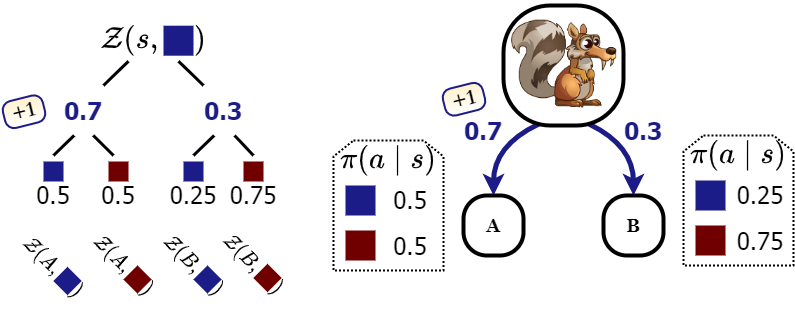
\includegraphics[width=1.1\textwidth]{Images/DistributionalBellmanExample.png}
\end{adjustwidth}
\end{exampleBox}

Подобные уравнения называются \emph{recursive distributional equations} и рассматриваются математикой в одном из разделов теории вероятности. Нам далее не понадобится какая-то особая теория оттуда, однако для вдохновения рассмотрим каноничный местный пример. 
\begin{example}
Пусть
$$X_1 \cdfeq \frac{X_2}{\sqrt{2}} + \frac{X_3}{\sqrt{2}}$$
где $X_1, X_2, X_3$ --- независимые случайные величины из одного распределения $p(x)$. То есть заданы две процедуры порождения: мы можем взять сэмпл из распределения, а может взять два сэмпла из распределения (независимо), отмасштабировать на корень из двух и сложить. Уравнение заявляет, что эти две процедуры эквивалентны. Вопрос для математики такой: каким могло бы быть $p(x)$? Несколько ответов можно угадать: например, ответом является, детерминированный ноль или $\N(0, \sigma^2)$.
\end{example}

\subsection{Distributional Policy Evaluation}

Будем строить аналог Policy Evaluation для distributional-формы оценочной функции. Иными словами, мы хотим чисто теоретический алгоритм, позволяющий для данного MDP и данной стратегии $\pi$ посчитать распределение $\Z^\pi(s, a)$. MDP пока считаем полностью известным (распределение $p(s' \mid s, a)$ считаем данным). Действуем в полной аналогии с обычными уравнениями: начнём с ввода оператора Беллмана.

\begin{definition}
Для данного MDP и стратегии $\pi$ будем называть \emph{оператором Беллмана в distributional форме} оператор $\B_D$, действующий из пространства Z-функций \eqref{Zfunctionspace} в пространство Z-функций, задающий случайную величину для $s, a$ на выходе оператора как правую часть distributional уравнения Беллмана \eqref{ZZ}:
$$\left[\B_D \Z^\pi\right](s, a) \cdfcoloneqq r(s, a) + \gamma \Z^\pi(s', a'), \quad s' \sim p(s' \mid s, a), a' \sim \pi(a' \mid s')$$
\end{definition}

\begin{wrapfigure}{r}{0.3\textwidth}
\vspace{-0.5cm}
\centering
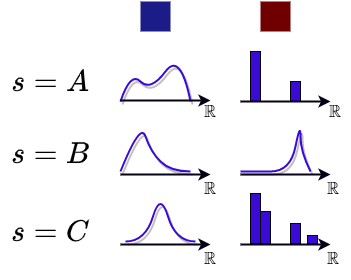
\includegraphics[width=0.3\textwidth]{Images/DistributionalTable.png}
\vspace{-0.9cm}
\end{wrapfigure}

Нас интересует вопрос о сходимости метода простой итерации. Что это означает? Если на $k$-ой итерации мы храним большую табличку, где для каждой пары $s, a$ хранится целиком и в точности всё распределение $\Z^\pi_k(s, a)$, то на очередном шаге для всех пар $s, a$ происходит обновление
\begin{equation}\label{distrpolicyevalupdate}
    \Z^\pi_{k+1}(s, a) \cdfcoloneqq r(s, a) + \gamma \Z^\pi_k(s', a'),
\end{equation}
где вероятности случайных величин $s' \sim p(s' \mid s, a), a' \sim \pi(a' \mid s')$ мы знаем и потому можем полностью посчитать свёртку распределений $\Z^{\pi}_k(s', a')$ для всевозможных пар следующих $s', a'$. 

Чтобы показать сходимость такой процедуры, хочется в аналогии с традиционным случаем доказать сжимаемость оператора $\B_D$. Однако, обсуждение сжимаемости имеет смысл только при заданной метрике, а в данном случае даже для конечных пространств состояний и пространств действий пространство Z-функций бесконечномерно, поскольку бесконечномерно $\Prob (\R)$. Нам нужна метрика в таком пространстве, и, внезапно, от её выбора будет зависеть ответ на вопрос о сжимаемости.

\begin{definition}
Пусть $\D$ --- метрика в пространстве $\Prob (\R)$. Тогда её \emph{максимальной формой} (maximal form) будем называть следующую метрику в пространстве Z-функций:
$$\D^{\max}(\Z_1, \Z_2) \coloneqq \sup\limits_{s \in \St, a \in \A} \D \left( \Z_1(s, a), \Z_2(s, a) \right)$$
\end{definition}

\begin{theorem}\label{constructmetric}
Для любой метрики $\D$ в пространстве $\Prob (\R)$ её максимальная форма $\D^{\max}$ есть метрика в пространстве Z-функций.
\begin{proof}
Проверим неравенство треугольника. Для любых трёх Z-функций $\Z_1, \Z_2, \Z_3$:
\begin{align*}
\D^{\max} (\Z_1, \Z_2) &= \sup\limits_{s, a} \D \left( \Z_1(s, a), \Z_2(s, a) \right) \le \\
\le \{ \text{неравенство треугольника для $\D$} \} &\le \sup\limits_{s, a} \left[ \D \left( \Z_1(s, a), \Z_3(s, a) \right) + \D \left( \Z_3(s, a), \Z_2(s, a) \right) \right] \le \\
\le \{ \text{свойство максимума} \} &\le \sup\limits_{s, a} \D \left( \Z_1(s, a), \Z_3(s, a) \right) + \sup\limits_{s, a} \D \left( \Z_3(s, a), \Z_2(s, a) \right) = \\
&= \D^{\max} (\Z_1, \Z_3) + \D^{\max} (\Z_3, \Z_2)
\end{align*}
Симметричность, неотрицательность и равенство нулю только при совпадении аргументов проверяется непосредственно.
\end{proof}
\end{theorem}

\begin{wrapfigure}{r}{0.3\textwidth}
\vspace{-0.5cm}
\centering
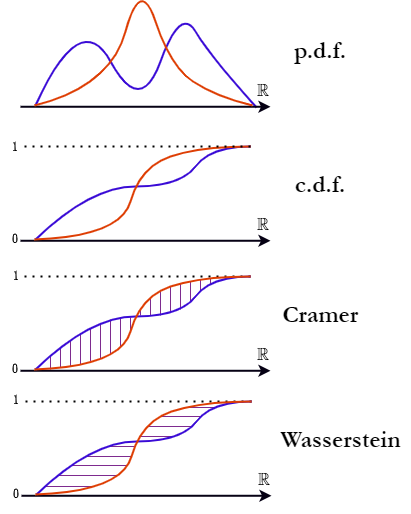
\includegraphics[width=0.3\textwidth]{Images/Wasserstein.png}
\vspace{-5.3cm}
\end{wrapfigure}

Соответственно, вопрос о выборе метрики в пространстве Z-функций сводится к вопросу о метрике в пространстве скалярных случайных величин. Вопрос, вообще, довольно богатый. Можно пытаться посчитать расстояние между функциями распределения (такова, например, \href{https://en.wikipedia.org/wiki/Energy_distance}{метрика Крамера}), а можно --- между их обратными функциями:

\begin{definition}
Для скалярной случайной величины $X$ с функцией распределения $F_X(x) \colon \R \to [0, 1]$ \emph{квантильной функцией} (inverse distribution function (quantile function)) называется\footnote{инфинум берётся для однозначности определения в ситуациях, когда в $F_X(x)$ есть плато.}
$$F^{-1}_X(\omega) \coloneqq \inf\{ x \in \R \mid F_X(x) \ge \omega \}$$
Значение этой функции $F^{-1}_X(\omega)$ в точке $\tau \in (0, 1)$ будем называть \emph{$\tau$-квантилем}. 
\end{definition}

\begin{definition}
Для $1 \le p \le +\infty$ для двух случайных скалярных величин\footnote{с ограниченными $p$-ми моментами, что в нашем контексте гарантируется ограниченностью награды \eqref{reward_limit} и ограниченностью домена.} $X, Y$ с функциями распределения $F_X$ and $F_Y$ соответственно \emph{расстоянием Вассерштайна} (Wasserstein distance) называется
\begin{equation}\label{wasserstein}
    \W_p(X, Y) \coloneqq \left( \int\limits_0^1 \left| F_X^{-1}(\omega) - F_Y^{-1}(\omega) \right| ^p \diff \omega \right)^{\frac{1}{p}}
\end{equation}
$$\W_\infty(X, Y) \coloneqq \sup_{\omega \in [0,1]} \left| F_X^{-1}(\omega) - F_Y^{-1}(\omega) \right| $$
\end{definition}

Расстояние Вассерштайна --- это довольно глубокая тема в математике; особый интерес представляет случай $p \HM= 1$ (см., например, \href{https://en.wikipedia.org/wiki/Wasserstein_metric}{википедию}). 

\begin{theorem}[Эквивалентная форма $\W_1$]
\begin{equation}\label{W1equiv}
\W_1(X, Y) = \int\limits_{\R} \left| F_X(x) - F_Y(x) \right| \diff x
\end{equation}
\beginproof
При $p \HM= 1$ расстояние Вассерштайна $\W_1$ есть просто площадь между графиками c.d.f. $F_X, F_Y$; тоже самое записано и в этой форме, только интегрирование (<<суммирование>>) проводится по оси значений, а не оси квантилей, но как график не поверни, площадь остаётся той же.

Формальное обоснование даёт теорема из матана о том, что в двойном интеграле можно менять местами интегралы:
$$ \int\limits_{\R} \left| F_X(x) - F_Y(x) \right| \diff x = \int\limits_{\R} \diff x \int\nolimits_{\min(F_X(x), F_Y(x))}^{\max(F_X(x), F_Y(x))} \diff \omega$$
Это площадь, если просуммировать вдоль оси $x$; давайте попробуем поменять местами интегралы. 

Рассмотрим какое-нибудь $\omega$; есть два симметричных случая. В первом $F_X(x) \le \omega \le F_Y(x)$. Ну тогда из второго неравенства $F_Y^{-1}(\omega) \le x$. Теперь заметим, что $F^{-1}_X(\omega) \ge F^{-1}_X(\hat{\omega})$ для любого $\hat{\omega} \le \omega$ в силу неубывания $F^{-1}_X$; поэтому возьмём в качестве $\hat{\omega} \coloneqq F_X(x)$, который по первому неравенству не больше $\omega$, и получим 
$$F^{-1}_X(\omega) \ge F^{-1}_X(\hat{\omega}) = F^{-1}_X(F_X(x)) = x$$
Мы получили, что $F^{-1}_X(\omega) \le x \le F^{-1}_Y(\omega)$. В симметричном случае, когда $F_Y(x) \le \omega \le F_X(x)$, мы получили бы аналогично $F^{-1}_Y(\omega) \le x \le F^{-1}_X(\omega)$. Таким образом, при данном $\omega$ для подсчёта площади переменной $x$ нужно пробежать от $\min(F^{-1}_X(x), F^{-1}_Y(x))$ до $\max(F^{-1}_X(x), F^{-1}_Y(x))$; мы получаем равенство
$$ \left( \int\limits_{\R} \diff x \int\nolimits_{\min(F_X(x), F_Y(x))}^{\max(F_X(x), F_Y(y))} \diff \omega \right) = \left( \int\limits_0^1 \diff \omega \int\nolimits_{\min(F^{-1}_X(\omega), F^{-1}_Y(\omega))}^{\max(F^{-1}_X(\omega), F^{-1}_Y(\omega))} \diff x \right)$$
Ну а это в точности равно $\W_1$, то есть выинтегрированию модуля разности между $F^{-1}_X$ и $F^{-1}_Y$.\qed

\beginproof[Замечание] Утверждение верно только для $p \HM= 1$: иначе существенно, вдоль какой оси мы растягиваем разность функций возведением в $p$-ую степень (физический смысл <<площади между графиками>> пропадает). Поэтому метрика Крамера, которая есть L2-расстояние между c.d.f., не равна $\W_2$, которая есть L2-расстояние между квантильными функциями.
\end{theorem}

\begin{exampleBox}[label=ex:emd]{}
Расстояние $\W_1$ между двумя распределениями неспроста имеет второе название \emph{Earth Moving Distance}. Аналогия такая: нам даны две кучи песка. Объём песка в кучах одинаков, но у них разные конфигурации, они <<насыпаны>> по-разному. Чтобы перенести каждую песчинку массы $m$ на расстояние $x$, нам нужно затратить <<работы>> объёмом $mx$. Расстояние Вассерштайна $\W_1$ замеряет, какое минимальное количество работы нужно совершить, чтобы перевести конфигурацию первой кучи песка во вторую кучу; объём песка в каждой кучи одинаков. Для дискретных распределений, когда функции распределения (и, соответственно, квантильные функции) --- <<ступеньки>>, минимальная работа полностью соответствует площади между функциями распределений.

\needspace{7\baselineskip}
\begin{wrapfigure}{r}{0.35\textwidth}
\vspace{-0.3cm}
\centering
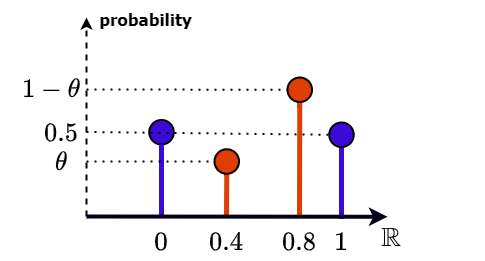
\includegraphics[width=0.35\textwidth]{Images/WassersteinSamples.png}
\vspace{-0.6cm}
\end{wrapfigure}
Посчитаем $\W_1$ между двумя следующими распределениями. Первое распределение (синие на картинке) --- честная монетка с исходами 0 и 1. Вторая случайная величина (красная на картинке) принимает значение 0.4 с вероятностью $\theta \HM< 0.5$ и 0.8 с вероятностью $1 \HM- \theta$. Можно нарисовать функции распределения и посчитать площадь между ними. А можно рассуждать так: давайте <<превратим>> вторую кучу песка в первую. Посмотрим на песок объёма $\theta$ в точке 0.4. Куда его переносить? Наверное, в точку 0, куда его тащить ближе. Перенесли; совершили работы объёмом $0.4\theta$. Посмотрим на песок объёма $1 \HM- \theta$ в точке 0.8. Его удобно тащить в точку 1, но там для получения первой конфигурации нужно только 0.5 песка. Поэтому 0.5 песка из точки 0.8 мы можем перевести в точку 1, совершив работу $0.2 \cdot 0.5$, а оставшийся объём $1 \HM- \theta \HM- 0.5$ придётся переводить в точку 0, совершая работу $0.8 (0.5 \HM- \theta)$. Итого расстояние Вассерштайна равно:
$$\W_1 = 0.4\theta + 0.8(0.5 - \theta) + 0.1$$
\end{exampleBox}

\begin{proposition}
Максимальная форма метрики Вассерштайна $\W^{\max}_p$ есть метрика в пространстве Z-функций.
\end{proposition}

\begin{theorem}
По метрике $\W^{\max}_p(\Z_1, \Z_2)$ оператор $\B_D$ является сжимающим.
\beginproof[Доказательство для $\W_1$] Воспользуемся формой расстояния через c.d.f. \eqref{W1equiv}, тогда
$$\W^{\max}_1(\B_D\Z_1, \B_D\Z_2) = \sup_{s, a} \int\limits_{\R} \left| \Prob(r + \gamma \Z_1(s', a') \le x) - \Prob(r + \gamma \Z_2(s', a') \le x) \right| \diff x = (*)$$
где внутри вероятностей $s', a'$ --- тоже случайные величины! Ну, сначала заметим, что добавление награды не изменяет значение интеграла. Давайте сделаем такую замену: $\hat{x} = \frac{x - r}{\gamma}$. Получаем:
$$(*) = \sup_{s, a} \gamma \int\limits_{\R} \left| \Prob(\Z_1(s', a') \le \hat{x}) - \Prob(\Z_2(s', a') \le \hat{x}) \right| \diff \hat{x} = (**)$$
Осталось справиться со случайностью $s', a'$; к счастью, для функций распределений это несложно. Пусть $s, a$ --- фиксированы, тогда просто по формуле полной вероятности:
$$\Prob(\Z(s', a') \le \hat{x}) = \int\limits_{\St} \int\limits_{\A} p(s' \mid s, a)\pi(a' \mid s') F_{\Z(s', a')}(\hat{x}) \diff s' \diff a',$$
где $F_{\Z(s', a')}(\hat{x})$ --- вероятность, что $\Z(s', a')$ не превзойдёт $\hat{x}$ при фиксированных $s', a'$. Подставляем:
\begin{align*}
(**) &= \gamma \sup_{s, a} \int\limits_{\R} \left| \int\limits_{\St} \int\limits_{\A} p(s' \mid s, a)\pi(a' \mid s') \left(F_{\Z_1(s', a')} - F_{\Z_2(s', a')} \right) \diff s' \diff a' \right| \diff \hat{x} \le \\
&\le \{ \text{наше любимое $\E_{x} f(x) \le \max\limits_x f(x)$} \} \le \gamma \sup_{s, a} \W^{\max}_1(\Z_1, \Z_2)   \tagqed
\end{align*}
\end{theorem}

Мы показали, что для систем уравнений \eqref{ZZ} выполняется теорема Банаха \ref{Banach}!

\begin{proposition}
Существует единственная функция $\St \times \A \to \Prob (\R)$, являющаяся решением уравнений \eqref{ZZ}, и метод простой итерации сходится к ней из любого начального приближения по метрике Вассерштайна.
\end{proposition}

\begin{example}
Попробуем угадать $\Z^{\pi}$ для случайной $\pi$ (выбирающей из двух действий всегда равновероятно) для MDP с рисунка и $\gamma \HM = 0.5$.

\needspace{7\baselineskip}
\begin{wrapfigure}{r}{0.15\textwidth}
\vspace{-0.5cm}
\centering
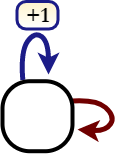
\includegraphics[width=0.12\textwidth]{Images/DistributionalExample.png}
\vspace{-0.3cm}
\end{wrapfigure}

Сначала попробуем понять, в каких границах может лежать наша награда. Если, например, мы всё время выбираем \colorsquare{ChadRed}, то получим в итоге ноль; меньше, понятно, получить нельзя. Аналогично если мы всё время выбираем \colorsquare{ChadBlue}, то получим в итоге $1 \HM+ \gamma \HM+ \gamma^2 \HM+ \dots \HM+ \HM= \frac{1}{1 - \gamma} \HM= 2$. Значит, вероятные исходы размазаны на отрезке $[0, 2]$. Есть ли среди этих исходов какие-то, которые имеют вероятность не ноль? Видимо, нет: то есть итоговое распределение награды какое-то непрерывное.

Попробуем подставить в уравнения Беллмана \eqref{ZZ} в качестве $\Z^{\pi}(\text{\colorsquare{ChadBlue}})$ равномерное распределение на отрезке $[1, 2]$ (так как гарантированно мы получим +1 на первом же шаге), а в качестве $\Z^{\pi}(\text{\colorsquare{ChadRed}})$ равномерное распределение на отрезке $[0, 1]$ (так как мы гарантированно получим не больше 1 за дальнейшую игру). Что мы получим? Вот мы выбрали $\colorsquare{ChadBlue}$: с одной стороны мы сказали, что получим равномерное из $[1, 2]$. С другой стороны можем рассмотреть <<одношаговую процедуру>>: мы точно получим +1, затем кинем кубик: с вероятностью 0.5 выберем на следующем шаге \colorsquare{ChadBlue} и получим равномерное из $[1, 2]$, а с вероятностью 0.5 выберем \colorsquare{ChadRed} и получим равномерное из $[0, 1]$. Значит, начиная со второго шага мы получим сэмпл из равномерного на $[0, 2]$; он будет дисконтирован на гамму и получится сэмпл из $[0, 1]$; дальше мы его сдвинем на +1, который мы получили на первом шаге, и в итоге как раз получится равномерное из $[1, 2]$! Сошлось; аналогично проверяется, что сходится второе distributional-уравнение. Из доказанного нами свойства сжатия следует, что это решение --- единственное, и является истинной $\Z^{\pi}$. 
\end{example}

Итак, мы с каждым шагом алгоритма становимся всё ближе к $\Z^\pi$, однако только если мы понимаем близость в терминах Вассерштайна. Это не единственная метрика в $\Prob ( \R )$, по максимальной форме которой была доказана сжимаемость $\B$; например, ещё она доказана для максимальной формы метрики Крамера. Важно, что есть примеры метрик, для максимальных форм которых свойства сжатия нет (например, \href{https://en.wikipedia.org/wiki/Total_variation_distance_of_probability_measures}{Total Variation}). Для нас важен более практический пример: в реальности нам с Вассерштайном обычно неудобно работать, и мы предпочитаем более удобные \emph{дивергенции}\footnote{снимается требование симметричности и неравенства треугольника.}, например, $\KL$-дивергенцию. Чисто теоретически мы можем задаться вопросом, как ведёт себя расстояние от $\Z_k \HM\coloneqq \B_D^k \Z^\pi_0$ до истинной $\Z^{\pi}$ в терминах KL-дивергенции, то есть стремится ли оно хотя бы к нулю? Оказывается, не просто не стремится, а вообще полное безобразие происходит: KL-дивергенция не умеет адекватно мерить расстояние между распределениями с \emph{несовпадающим доменом} (disjoint support).

\begin{theorem}
Расстояние между $\B_D^k \Z^\pi_0$ и истинным $\Z^\pi$ по максимальной форме $\KL$-дивергенции может быть равно бесконечности для всех $k$.

\needspace{7\baselineskip}
\begin{wrapfigure}{r}{0.2\textwidth}
\vspace{-1cm}
\centering
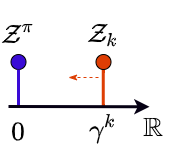
\includegraphics[width=0.2\textwidth]{Images/KLdivProblem.png}
\vspace{-0.5cm}
\end{wrapfigure}
\beginproof[Пример]
Пусть в MDP с одним состоянием, одним действием и нулевой функцией награды мы проинициализировали $\Z^\pi_0$ вырожденной случайной величиной, всегда принимающей значение 1. Тогда на первом шаге метода мы получим случайную величину, с вероятностью 1 равную $\gamma$; на $k$-ом шаге, по индукции, случайную величину, с вероятностью 1 равную $\gamma^k$. При этом $\KL$-дивергенция между ней и истинным распределением $\Z^\pi$ --- вырожденной в нуле --- равна бесконечности! \qed
\end{theorem}

Так, ну ладно: оно же сходится по Вассерштайну, который лишён этой проблемы. Мы показали, что мы чисто теоретически умеем конструктивно находить $\Z^{\pi}$, запустив метод простой итерации из произвольного начального приближения (в том числе, кстати, можем стартовать из вырожденных распределений). От практического алгоритма нас пока отделяет тот факт, что даже в табличном сеттинге мы не умеем в ячейках таблицы хранить <<полностью>> распределения на $\R$; мы займёмся этой проблемой чуть позже.

Пока что ответим на такой вопрос: а вот когда мы учим так $\Z^{\pi}$, что там происходит с их мат.ожиданиями, то есть, по сути, с нашими представлениями о $Q^\pi$? Может, они там как-то быстрее сходятся за счёт того, что мы начали дополнительную информацию о распределении учить? Нет: их поведение в точности совпадает с тем, что получилось бы в методе простой итерации для обучения Q-функции непосредственно.

Пусть $\B$ --- обычный оператор Беллмана из пространства Q-функций в пространство Q-функций, а $\B_D$, как и раньше, оператор Беллмана из пространства Z-функций в пространство Z-функций.

\begin{theorem}
Пусть инициализации $\Z^\pi_0$ и $Q^\pi_0$ удовлетворяют $\E \Z^\pi_0 = Q^\pi_0$, и рассматривается два метода простой итерации:
$$Q^\pi_k \coloneqq \B^k Q^\pi_0$$
$$\Z^\pi_k \coloneqq \B_D^k \Z^\pi_0$$
Тогда:
$$Q^\pi_k = \E \Z^\pi_k$$
\beginproof
По индукции. Пусть это верно для $k$-ой итерации, покажем для $k+1$-ой:
$$\E \Z^\pi_{k+1} = \E \left[ \B_D \Z^\pi_k \right](s, a) = \E r(s, a) + \gamma \Z^\pi_k(s', a') = (*)$$
Заметим, что мат.ожидание в последнем выражении берётся по $s', a'$ и случайности в $\Z^\pi_k(s', a')$ (случайности по хвосту траектории). По предположению индукции:
$$\E \Z^\pi_k(s', a') = Q^\pi_k(s', a')$$
Подставляем:
\begin{align*}
(*) =  \E_{s'} \E_{a'} r(s, a) + \gamma \E \Z^\pi_k(s', a') = \E_{s'}\E_{a'} \left[ r(s, a) + \gamma Q^\pi_k(s', a') \right] = \B Q^\pi_k = Q^\pi_{k+1}   \tagqed
\end{align*}
\end{theorem}

\subsection{Distributional Value Iteration}

По аналогии с традиционным случаем, очень хочется ввести оптимальную оценочную функцию в distributional-форме как Z-функцию оптимальных стратегий:
\begin{equation}\label{optimalZ}
\Z^*(s, a) \cdfcoloneqq Z^{\pi^*}(s, a)
\end{equation}

Мы начинаем спотыкаться уже на этом моменте, и дальше будет только хуже.

\begin{theorem}
Определение \eqref{optimalZ} неоднозначно.

\needspace{7\baselineskip}
\begin{wrapfigure}{r}{0.25\textwidth}
\vspace{-1cm}
\centering
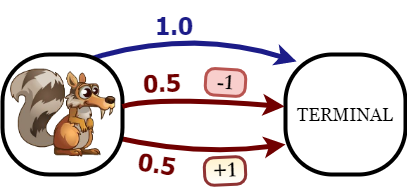
\includegraphics[width=0.25\textwidth]{Images/optimalZissue.png}
%\vspace{-0.6cm}
\end{wrapfigure}
\beginproof
Рассмотрим MDP, где агент может выбрать действие $a \HM= \colorsquare{ChadBlue}$ и получить нулевую награду с вероятностью 1, или $a \HM = \colorsquare{ChadRed}$ и получить +1 или -1 с вероятностями 0.5 (эпизод в обоих случаях заканчивается). Все стратегии будут оптимальными, хотя все Z-функции различны. \qed
\end{theorem}

С уравнением оптимальности Беллмана для $\Z^*$ тоже внезапно есть тонкости. Для любой оптимальной стратегии  $\pi^*$ вследствие \eqref{QZ} верно, что
$$Q^*(s, a) = \E \Z^{\pi^*}(s, a),$$
и мы знаем, что, в частности, среди оптимальных есть стратегия
$$\pi^*(s) = \argmax\limits_a Q^*(s, a) = \argmax\limits_a \E \Z^{\pi^*}(s, a).$$
В принципе, можно взять \eqref{ZZ} для этой $\pi^*(s)$ и использовать её вид.
\begin{equation}\label{Z*Z*}
\Z^*(s, a) \cdfeq r(s, a) + \gamma \Z^*(s', \pi^*(s')), \quad s' \sim p(s' \mid s, a)
\end{equation}
Здесь справа мы для данных $s, a$ описываем следующий процесс генерации случайной величины: генерируем $s'$ из функции переходов, определяем однозначно\footnote{здесь есть нюанс с выбором жадного действия в случае равного среднего для нескольких вариантов: для полной корректности, множество действий должно быть упорядочено, и в <<спорных>> ситуациях следует выбирать действие с наименьшим порядком. Это существенно, поскольку выбор разных оптимальных действий приводит к одному и тому же среднему, но другие статистики могут быть различны.} $a' = \argmax\limits_{a'} \E \Z^*(s', a')$, после чего генерируем сэмпл $\Z^*(s', a')$ и выдаём $r(s, a) + \gamma \Z^*(s', a')$ в качестве результата.

Заметим, что взятие мат.ожидания справа и слева в уравнении \eqref{Z*Z*} приведёт к традиционному уравнению оптимальности Беллмана для Q \eqref{Q*Q*}.

\begin{definition}
Введём \emph{оператор оптимальности Беллмана в distributional-форме} $\B^*_D$:
$$\left[\B^*_D \Z^* \right] (s, a) \cdfcoloneqq r(s, a) + \gamma \Z^*(s', \argmax\limits_{a'} \E \Z^*(s', a')), \quad s' \sim p(s' \mid s, a)$$
\end{definition}

Пусть также $\B^*$ --- обычный оператор оптимальности Беллмана из пространства Q-функций в пространство Q-функций.

\begin{theoremBox}[label=th:distributionalVIiscorrect]{}
Пусть инициализации $\Z^*_0$ и $Q^*_0$ удовлетворяют $\E \Z^*_0 = Q^*_0$ и рассматривается два метода простой итерации:
$$Q^*_k \coloneqq \left(\B^*\right)^k Q^*_0$$
$$\Z^*_k \coloneqq \left(\B^*_D\right)^k \Z^*_0$$
Тогда:
$$Q^*_k = \E \Z^*_k$$
\beginproof
По индукции. Пусть это верно для $k$-ой итерации, покажем для $k+1$-ой:
$$\E \Z^*_{k+1} = \E \left[ \B^*_D \Z^*_k \right](s, a) = \E \left[ r(s, a) + \gamma \Z^*_k(s', \argmax\limits_{a'} \E \Z^*_k(s', a')) \right] = (*)$$
Заметим, что внутренний аргмакс эквивалентен аргмаксу по $Q$-функции, так что здесь мы тоже можем воспользоваться предположением индукции:
$$\E \Z^*_k(s', a') = Q^*_k(s', a')$$
Подставляем:
\begin{align*}
(*) &= \E_{s'}\E_{a'} \left[ r(s, a) + \gamma \E \Z^*_k(s', \argmax\limits_{a'} Q^*_k(s', a')) \right] = \\ 
&= r(s, a) + \gamma Q^*_k(s', \argmax\limits_{a'} Q^*_k(s', a')) = \\
&= r(s, a) + \gamma \max\limits_{a'} Q^*_k(s', a') = \B^* Q^*_k = Q^*_{k+1}   \tagqed
\end{align*}
\end{theoremBox}

Итак, мы показали, что в методе простой итерации с оператором $\B^*_D$ средние движутся точно также, как и $Q^*$ в обычном подходе. Однако, хвосты распределений при этом могут вести себя довольно нестабильно, и понятно, почему.

\begin{theorem}
Оператор $\B^*_D$ может не являться непрерывным.

\needspace{13\baselineskip}
\begin{wrapfigure}{r}{0.3\textwidth}
\vspace{-1cm}
\centering
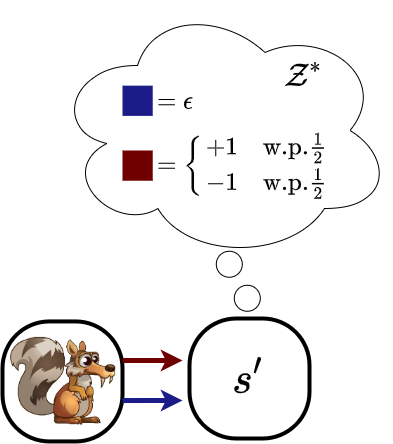
\includegraphics[width=0.28\textwidth]{Images/distributionalVIissue.png}
\vspace{0.2cm}
\end{wrapfigure}
\beginproof
Пусть после выполнения $s, a$ мы точно попадаем в некоторое $s'$, для которого наше приближение $\Z^*$ указано как на рисунке; варьируя $\epsilon$, мы можем получать близкие (по любой непрерывной метрике) Z-функции. Рассмотрим $\epsilon \HM\to 0$ и поймём, что оператор $\B^*_D$ выдаёт совершенно разные Z-функции в зависимости от того, приближаемся ли мы к нулю с положительной полуоси или отрицательной.

Смотрим на $\left[ \B^*_D \Z \right](s, a) \HM\cdfcoloneqq \Z(s', \pi^*(s'))$, где $\pi^*(s')$ --- жадная. Если $\epsilon \HM> 0$, жадная политика выдаст $a' \HM= \text{\colorsquare{ChadBlue}}$, и результат оператора будет вырожденным, а если $\epsilon \HM< 0$, то результат оператора будет дискретным распределением с двумя атомами $\gamma$ и $-\gamma$. Расстояние между этими двумя вариантами по любой метрике не будет нулевым. Иными словами, при переходе $\epsilon$ через ноль при непрерывном изменении аргумента оператора значение оператора может сколько угодно сильно измениться. \qed
\end{theorem}

\begin{proposition}
Оператор $\B^*_D$ может не являться сжимающим.
\begin{proof}[Пояснение] По определению, любой сжимающий оператор \href{https://ru.wikipedia.org/wiki/\%D0\%9B\%D0\%B8\%D0\%BF\%D1\%88\%D0\%B8\%D1\%86\%D0\%B5\%D0\%B2\%D0\%BE_\%D0\%BE\%D1\%82\%D0\%BE\%D0\%B1\%D1\%80\%D0\%B0\%D0\%B6\%D0\%B5\%D0\%BD\%D0\%B8\%D0\%B5}{Липшицев}, и, значит, обязан быть непрерывным.
\end{proof}
\end{proposition}

Мы, тем не менее, показали, что средние сходятся к $Q^*$, поэтому не совсем ясно, насколько страшно, что хвосты распределений могут начать вести как-то нестабильно.

\subsection{Категориальная аппроксимация Z-функций}

Пока что мы не получили даже табличный алгоритм в рамках distributional-подхода: даже если пространства $\St$ и $\A$ конечны, а функция переходов известна, хранить в памяти точное распределение $\Z^*(s, a)$ мы не умеем. Нам придётся выбрать некоторую параметрическую аппроксимацию. Хорошая новость заключается в том, что награда --- скаляр, и распределения, с которыми мы хотим работать, одномерны. Более того, в силу \eqref{reward_limit} домен распределений ограничен. Мы можем этим воспользоваться и придумать какую-нибудь <<сеточную>> аппроксимацию.

\begin{definition}
Зададимся набором \emph{атомов} (atoms) $r^{\min} = z_0 \HM< z_1 \HM< z_2 \dots < z_A = r^{\max}$, где $A + 1$ --- число атомов. Обозначим \emph{семейство категориальных распределений} $\mathcal{C} \subset \Prob(\R)$ как множество дискретных распределений на домене $\{z_0, z_1 \dots z_A\}$: если $\Z^*(s, a) \in \mathcal{C}$, то
$$\Prob \left( \Z^*(s, a) = z_i \right) = p_i,$$
где $p$ --- набор из 51 числа, суммирующихся в единицу.
\end{definition}

\begin{example}[c51]
Типично атомы образуют просто равномерную сетку, для задания которой требуется три гиперпараметра: число атомов $A$, минимальное и максимальное значение награды. Распространённый дефолтный вариант для Atari игр --- 51 атом на отрезке $[-10, 10]$.
\end{example}

\needspace{7\baselineskip}
\begin{wrapfigure}{r}{0.35\textwidth}
\vspace{-0.3cm}
\centering
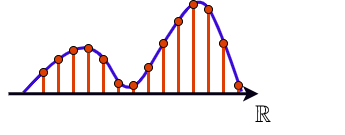
\includegraphics[width=0.35\textwidth]{Images/Categorical.png}
\vspace{-0.6cm}
\end{wrapfigure}
Итак, для каждой пары $s, a$ мы будем хранить в табличке $A + 1$ неотрицательное число $p_0, p_1 \dots p_A$, суммирующиеся в единицу, и полагать, что $A+1$ узлов нашей сетки $z_0, z_1 \dots z_A$ являются единственно возможными исходами будущей награды. Такова наша аппроксимация.

 Возникает следующая проблема: мы, в принципе, можем посчитать распределения $\B^*_D \Z^*$, но что, если оно <<не попадёт>> в рассматриваемое семейство аппроксимаций? То есть что, если для какой-то пары $s, a$ $[\B^*_D \Z^*](s, a) \not\in \mathcal{C}$, то есть если оно не является категориальным распределением на домене $\{z_0, z_1 \dots z_A\}$? Нам придётся как-то проецировать полученный результат на нашу сетку...
 
 \begin{proposition}
 Если $\Z(s, a) \in \mathcal{C}$ для всех $s, a$, то $\left[\B^*_D \Z\right](s, a)$ --- дискретное распределение с конечным множеством исходов.
 \begin{proof} Распределение является смесью не более чем $|\St| |\A|$ категориальных распределений с $A$ исходами, поэтому у него не может быть более $|\St| |\A| A$ различных исходов.
 \end{proof}
 \end{proposition}
 
 Значит, нам нужно научиться проецировать лишь дискретные распределения.
 
 \begin{definition}
 Введём \emph{оператор проекции} $\Pi$, действующий из пространства произвольных дискретных распределений в $\mathcal{C}$ следующим образом. Пусть $\tilde{\Z}(s, a)$ --- произвольное дискретное распределение с исходами $\tilde{z}_i$ с соответствующими вероятностями $\tilde{p}_i$ (суммирующимися в единицу). Изначально инициализируем все $p_i$ для результата работы оператора нулями.
 
 Дальше перебираем исходы $\tilde{z}_i$; если очередной исход меньше $r^{\min} \HM= z_0$, всю его вероятностную массу отправляем в $p_0$, то есть увеличиваем $p_0$ на $\tilde{z}_i$. Аналогично поступаем если $\tilde{z}_i \HM> r^{\max} = z_A$. В остальных случаях найдётся два соседних атома нашей сетки, такие что $z_j \HM\le \tilde{z}_i \HM\le z_{j+1}$. Распределим вероятностную массу между ними обратно пропорционально расстоянию до них, а то есть:
\begin{equation}\label{projector}
\begin{split} 
p_j \leftarrow p_j + \frac{z_{j+1} - \tilde{z}_i}{z_{j+1} - z_j} \tilde{p}_i  \\
p_{j+1} \leftarrow p_{j+1} + \frac{\tilde{z}_i - z_j}{z_{j+1} - z_j} \tilde{p}_i
\end{split}
\end{equation}
 \end{definition}

Почему именно так мы ввели оператор проекции? Наш метод простой итерации теперь <<подкорректированный>>, после каждого шага мы применяем проекцию:
$$\Z^*_{k+1} \cdfcoloneqq \Pi \B^*_D \Z^*_{k},$$
где применение $\Pi$ к Z-функции означает проецирование всех распределений $\Z(s, a)$ для всех $s, a$. Мы очень хотели бы сохранить гарантии теоремы \ref{th:distributionalVIiscorrect} о том, что средние в таком подправленном процессе продолжают вести себя как аппроксимации Q-функции в Value Iteration!

\begin{theorem}
Пусть $\Z(s, a)$ дискретно и выдаёт исходам вне отрезка $[r_{\min}, r_{\max}]$ нулевую вероятность. Тогда оператор проекции \eqref{projector} сохраняет мат.ожидание, $\forall \Z, s, a \colon$
$$\E \Pi \Z (s, a) = \E \Z(s, a)$$
 
\needspace{7\baselineskip}
\begin{wrapfigure}{r}{0.4\textwidth}
\vspace{-1cm}
\centering
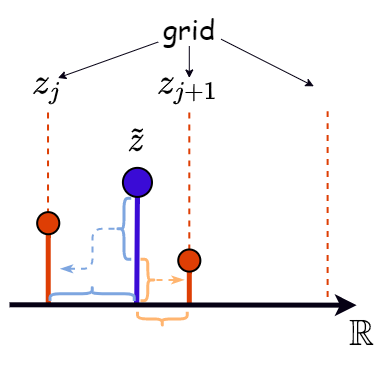
\includegraphics[width=0.4\textwidth]{Images/Projecting.png}
\vspace{-0.6cm}
\end{wrapfigure}
\beginproof
Рассмотрим один исход $\Z(s, a)$; он вносил в итоговое среднее вклад $\tilde{z}\tilde{p}$, где $\tilde{p}$ --- его вероятность, $\tilde{z}$ --- значение исхода. По условию, вся вероятностная масса размазывалась между двумя соседними узлами $z_j \le \tilde{z} \le z_{j+1}$, и в $\left[\Pi \Z\right](s, a)$ соответственно появляется два слагаемых:
\begin{align*}
    &\overbrace{\frac{z_{j+1} - \tilde{z}}{z_{j+1} - z_j} \tilde{p} z_j}^{\text{левый узел}} + \overbrace{\frac{\tilde{z} - z_j}{z_{j+1} - z_j} \tilde{p} z_{j+1}}^{\text{правый узел}} = \\ = &\frac{z_{j+1}z_j - \tilde{z}z_j + \tilde{z}z_{j+1} - z_{j}z_{j+1}}{z_{j+1} - z_j} \tilde{p} = \\ = &\tilde{z}\tilde{p}   \tagqed
\end{align*}
\end{theorem}

\subsection{Categorical DQN}\label{subsec:c51}

\needspace{7\baselineskip}
\begin{wrapfigure}{r}{0.3\textwidth}
\vspace{-0.5cm}
\centering
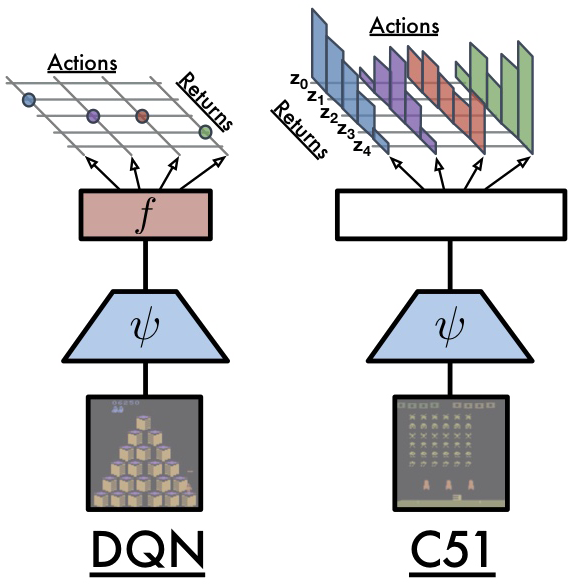
\includegraphics[width=0.3\textwidth]{Images/c51.png}
\vspace{-0.5cm}
\end{wrapfigure}
Попробуем составить уже полностью практический алгоритм. Во-первых, обобщим алгоритм на случай произвольных пространств состояний, моделируя $\Z^*$ (а точнее --- её распределение) при помощи нейросети. Для каждой пары $s, a$ нейросеть с параметрами $\theta$ выдаёт $A+1$ неотрицательное число $p_1(s, a, \theta), p_2(s, a, \theta) \dots p_A(s, a, \theta)$, суммирующиеся в единицу, и мы предполагаем категориальную аппроксимацию
$$\Prob \left( \Z^*(s, a, \theta) = z_i \right) \coloneqq p_i(s, a, \theta).$$
Как и в DQN, считаем, что у нас есть таргет-сеть с параметрами $\theta^{-}$ --- Z-функция $\Z^*_{\theta^-}$ с предыдущего (условно, $k$-го) шага метода простой итерации, а мы хотим обучать $\theta$ так, чтобы получить Z-функцию на $k+1$-ом шаге: наша цель --- выучить $\B^*_D \Z^*_{\theta^-}$. 

В model-free режиме, без доступа к функции переходов, мы не то чтобы посчитать $\B^*_D \Z^*_{\theta^-}$ не можем, нам даже недоступна большая часть информации о нём. Для данной пары $s, a$ из реплей буфера мы можем получить только один сэмпл $s' \sim p(s' \mid s, a)$, и нам нужен какой-то <<аналог>> метода временных разностей.

Первое соображение: мы умеем сэмплировать из $[\B^*_D \Z^*_{\theta^-}](s, a)$. Действительно: пусть дано $s, a$; берём сэмпл $s'$ из, например, буфера; смотрим на нашу таргет сеть $\Z^*_{\theta^-}(s', a')$ для всех действий $a'$, считаем у каждого мат.ожидание (для ситуации $\Z^*_{\theta^-}(s', a') \in \mathcal{C}$ это, очевидно, не проблема) и выбираем <<наилучшее>> действие $a' \HM= \argmax\limits_{a'} \E \Z^*_{\theta^-}(s', a')$. Выбираем такое $a'$, и дальше у нас есть даже не сэмпл, а целая компонента распределения $[\B^*_D \Z^*_{\theta^-}](s, a)$ в виде распределения $r(s, a) + \gamma \Z^*_{\theta^-}(s', a')$. 

Итак, пусть $\T \coloneqq (s, a, r, s', \done)$ --- пятёрка из буфера. Введём целевую переменную (таргет) следующим образом:
\begin{equation}\label{distributionaltarget}
y(\T) \cdfcoloneqq r + \gamma (1 - \done) \Z^*(s', \argmax_{a'} \E \Z^*(s', a', \theta^{-}), \theta^{-})
\end{equation}
где $s'$ в формуле берётся из $\T$, то есть взято из буфера. Такой таргет является дискретным распределением с, очевидно, $A$ атомами, но из-за того, что мы взяли лишь один сэмпл $s'$, он является лишь компонентой из $[\B^*_D \Z^*_{\theta^-}](s, a)$.

Второе соображение: допустим, для данной пары $s, a$ мы сможем оптимизировать следующий функционал для некоторой дивергенции $\D$, используя лишь сэмплы из первого распределения:
\begin{equation}\label{distributionalopt}
\D ([\B^*_D \Z^*_{\theta^-} ] (s, a) \parallel \Z^*(s, a, \theta)) \to \min_{\theta}
\end{equation}

Если бы мы могли моделировать произвольные Z-функции, минимум достигался бы в нуле на совпадающих распределениях, и наша цель была бы достигнута. Однако мы ограничены нашим аппроксимирующим категориальным семейством $\mathcal{C}$, и при оптимизации такого функционала даже чисто теоретически мы получим лишь проекцию на $\mathcal{C}$; здесь возникает вопрос, а не потеряем ли мы свойство сохранения мат.ожидания. Мы знаем, что наш оператор проекции \eqref{projector} обладает этим свойством: мы могли бы приближать наше распределение сразу к <<хорошей>> проекции:
$$\D ([\Pi \B^*_D \Z^*_{\theta^-}](s, a) \parallel \Z^*(s, a, \theta)) \to \min_{\theta}$$
Тогда мы будем учить категориальное распределение с сохранённым мат.ожиданием. 

Вопрос: не потеряли ли мы возможность сэмплировать из целевого распределения? То есть можем ли мы получить сэмпл из $[\Pi \B^*_D \Z^*_{\theta^-}](s, a)$?

\begin{theorem}
\begin{equation}\label{projectioncomponents}
[\Pi \B^*_D \Z^*_{\theta^-}](s, a) \cdfeq \Pi y(\T), \quad s' \sim p(s' \mid s, a)
\end{equation}
\beginproof[Пояснение]
Сначала разберёмся, что здесь написано. Мы можем (теоретически) посчитать полностью одношаговую аппроксимацию $\B^*_D \Z^*_{\theta^-}$ и спроецировать полученное распредление (случ. величина слева); а можем взять случайный $s'$, посмотреть на распределение $r + \gamma\Z^*_{\theta^-}(s', a')$ для жадного $a'$ и спроецировать его (случ. величина справа). Утверждается эквивалентность этих процедур: мы можем проецировать лишь компоненты $[\B^*_D \Z^*_{\theta^-}](s, a)$. Таким образом, сэмплы из $\Pi y(\T)$ при случайных $s' \sim p(s' \mid s, a)$ есть сэмплы $[\Pi \B^*_D \Z^*_{\theta^-}](s, a)$.

\begin{proof} Следует, в общем-то, из определения нашего оператора проекции \eqref{projector}, который с каждым возможным исходом работает <<независимо>> от всех остальных. Пусть для некоторого $s'$ $p$ --- вероятность исхода $z$, тогда в правой части эта вероятность будет размазана между соседними узлами $z_i \le z \le z_{i+1}$ с некоторыми весами $w_i, w_{i+1}$. Тогда в силу того, что $s'$ случайно, эта вероятностная масса в итоговом распределении в правой части уравнения будет домножена на $p(s' \mid s, a)$. В распределении в левой части вероятностная масса будет сначала домножена на $p(s' \mid s, a)$, а только потом размазана между теми же $z_i, z_{i+1}$ с теми же весами $w_i, w_{i+1}$ (которые по определению зависят только от значения исхода $z$); очевидно, эти процедуры эквивалентны.
% \begin{align*}
% \Prob (\Pi \B^*_D \Z^*_{\theta^-} = z_j) &= \int\limits_{z_{j}}^{z_{j+1}} \frac{z_{j+1} - \tilde{z}}{z_{j+1} - z_j} \Prob(\B^*_D \Z^*_{\theta^-} = \tilde{z}) \diff \tilde{z} + \int\limits_{z_{j - 1}}^{z_{j}} \frac{\tilde{z} - z_{j-1}}{z_{j} - z_{j-1}} \Prob(\B^*_D \Z^*_{\theta^-} = \tilde{z}) \diff \tilde{z} = \\
% &= \int\limits_{z_{j}}^{z_{j+1}} \frac{z_{j+1} - \tilde{z}}{z_{j+1} - z_j}  \int_{\St} p(s' \mid s, a) \Prob(y(\T) = \tilde{z}) \diff \tilde{z} \diff s' + \int\limits_{z_{j - 1}}^{z_{j}} \frac{\tilde{z} - z_{j-1}}{z_{j} - z_{j-1}} \int_{\St} p(s' \mid s, a) \Prob(y(\T) = \tilde{z}) \diff \tilde{z} \diff s'  = \\
% &= \int_{\St} p(s' \mid s, a) \left[ \int\limits_{z_{j}}^{z_{j+1}} \frac{z_{j+1} - \tilde{z}}{z_{j+1} - z_j} \Prob(y(\T) = \tilde{z}) \diff \tilde{z} + \int\limits_{z_{j - 1}}^{z_{j}} \frac{\tilde{z} - z_{j-1}}{z_{j} - z_{j-1}} \Prob(y(\T) = \tilde{z})  \diff \tilde{z} \right] \diff s' = \\
% &= \int_{\St} p(s' \mid s, a) \Prob(\Pi y(\T) = z_j \mid s') \diff \tilde{z} = \\
% &= \Prob(\Pi y(\T) = z_j)
% \end{align*}
\end{proof}
\end{theorem}

Итак, $\Pi y(\T)$ есть компонента $[\Pi \B^*_D \Z^*_{\theta^-}](s, a)$, то есть у нас, условно, есть сэмплы из этого распределения. Для каких метрик $\D$ мы умеем получать несмещённую оценку градиента \eqref{distributionalopt} по сэмплам? Теория подсказывает, что в пространстве Z-функций осмысленной метрикой является Вассерштайн \eqref{wasserstein}. И тут случается облом.

\begin{theorem}
Градиенты расстояния Вассерштайна до сэмплов не являются несмещёнными оценками градиента расстояния Вассерштайна до полного распределения.

\needspace{7\baselineskip}
\begin{wrapfigure}{r}{0.35\textwidth}
\vspace{-0.3cm}
\centering
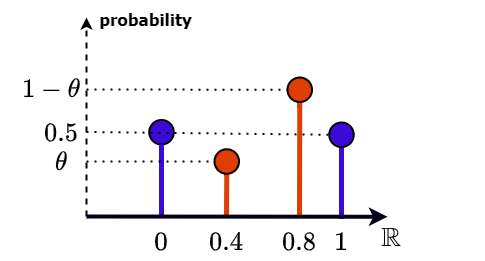
\includegraphics[width=0.35\textwidth]{Images/WassersteinSamples.png}
\vspace{-0.6cm}
\end{wrapfigure}
\beginproof[Контрпример]
Контрпримером будет являться практически любая ситуация, где $s'$ недетерминировано, а наше параметрическое семейство $\Z^*_{\theta}$ может моделировать невырожденные случайные величины; так в принципе устроено расстояние Вассерштайна.

Разберём какой-нибудь пример, для простоты для $\W_1$. Пусть для данных $s, a$ с вероятностью 0.5 $s'$ такого, что $y_1(\T)$ --- вырожденная в нуле, а с вероятностью 0.5 $s'$ такого, что $y_2(\T)$ --- вырожденная в единице. Тогда понятно, что целиком распределение $[\B^*_D \Z^*_{\theta^-}](s, a)$ есть распределение с двумя равновероятными исходами, 0 и 1. 

Пусть $\Z_{\theta}$ равна 0.4 с вероятностью $\theta$ и 0.8 с вероятностью $1 \HM- \theta$, других значений не принимает. Будем смотреть на точку $\theta < 0.5$. Мы как раз считали подобные расстояния Вассерштайна в примере \ref{ex:emd}. Тогда:
$$\W_1 \left( \B^*_D \Z^*_{\theta^-}(s, a) \parallel \Z_{\theta} \right) = 0.4\theta + 0.8(0.5 - \theta) + 0.1$$
$$\W_1 \left( y_1(\T) \parallel \Z_{\theta} \right) = 0.4 \theta + 0.8 (1 - \theta)$$
$$\W_1 \left( y_2(\T) \parallel \Z_{\theta} \right) = 0.6 \theta + 0.2 (1 - \theta)$$
Получаем:
$$\nabla_\theta \W_1 \left( [\B^*_D \Z^*_{\theta^-})] \parallel \Z_{\theta} \right) = -0.4\theta$$
$$\nabla_\theta \E_{s'} \W_p \left( y(\T) \parallel \Z_{\theta} \right) = \frac{1}{2} (-0.4\theta) + \frac{1}{2} (0.4\theta) = 0$$
Не сходится. \qed
\end{theorem}

Как мы сейчас покажем, псевдометрикой, которую можно оптимизировать по сэмплам, является наша любимая KL-дивергенция. Мы понимаем, что, с одной стороны, теория подсказывает нам, что в пространстве Z-функций $\KL$-дивергенция потенциально не приближает нас к истинной оптимальной Z-функции, но зато мы сможем оптимизировать её в model-free режиме.

Итак, рассмотрим в \eqref{distributionalopt} в качестве $\D$ $\KL$-дивергенцию (значит, будет важен порядок аргументов). Для неё вылезает ещё одна проблема: домен сравниваемых распределений должен совпадать, иначе KL-дивергенция по определению бесконечность и не оптимизируется. К счастью, мы уже решили, что мы будем в качестве целевого распределения использовать $\Pi y(\T)$, которое имеет тот же домен --- сетку $z_0 \HM< z_1 \HM< \dots \HM< z_A$. 

\begin{theorem}
Градиент $\KL$-дивергенции до целевой переменной $\Pi y(\T)$ есть несмещённая оценка градиента \eqref{distributionalopt}:
\begin{equation}\label{c51loss}
\nabla_\theta \KL (\Pi \B^*_D \Z^*_{\theta^-}(s, a) \parallel \Z^*(s, a, \theta)) = \E_{s'} \nabla_\theta \KL (\Pi y(\T) \parallel \Z^*(s, a, \theta))
\end{equation}
\beginproof
\begin{align*}\nabla_\theta \KL (\Pi \B^*_D \Z^*_{\theta^-}(s, a) \parallel \Z^*(s, a, \theta)) &= \nabla_\theta \const(\theta) - \\
&- \nabla_\theta \E_{z \sim \Pi \B^*_D \Z_{\theta^-}^*(s, a)} \log \Prob \left( \Z^*(s, a, \theta) = z \right) = \\
= \{ \text{\eqref{projectioncomponents}} \} &= -\nabla_\theta \E_{s'} \E_{z \sim \Pi y(\T)} \log \Prob \left( \Z^*(s, a, \theta) = z \right) = \\
&=\E_{s'} \nabla_\theta \KL (\Pi y(\T) \parallel \Z^*(s, a, \theta))     \tagqed
\end{align*}
\end{theorem}

\needspace{14\baselineskip}
\begin{wrapfigure}{r}{0.4\textwidth}
%\vspace{-0.3cm}
\centering
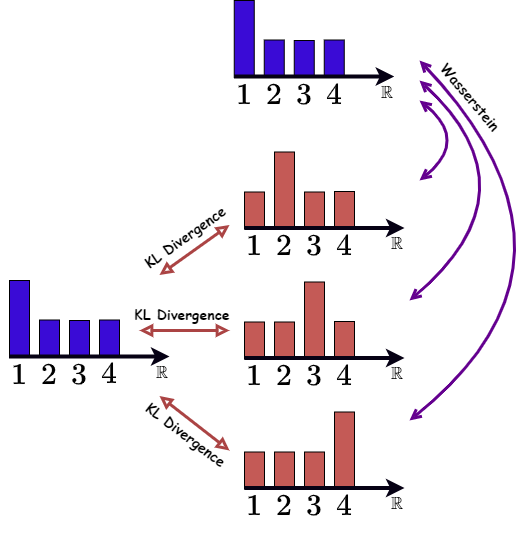
\includegraphics[width=0.4\textwidth]{Images/KLgeometry.png}
\vspace{-0.8cm}
\end{wrapfigure}

Итак, градиент KL-дивергенции --- мат.ожидание по целевому распределению, и значит, мы можем вместо мат.ожидания по $\Pi \B^*_D \Z^*(s, a, \theta^-)$ использовать Монте-Карло оценку по сэмплам. При этом поскольку у нас есть даже не просто сэмплы, а целая компонента $\Pi y(\T)$ целевого распределения, то по ней интеграл мы можем взять просто целиком (он состоит всего из $A$ слагаемых, как видно, поскольку $\Pi y(\T) \in \mathcal{C}$).

Мы по сути, как видно из формулы \eqref{c51loss}, начинаем решать задачу классификации, где у нас есть для данного входа $s, a$ сразу целая компонента распределения целевой переменной. Минимизация KL-дивергенции, хоть и является стандартной функций потерь в таких ситуациях, сейчас имеет для нас побочный эффект: мы отчасти потеряли <<физический смысл>> наших <<классов>>. KL-дивергенция смотрит на каждый узел $z_i$ нашей сетки отдельно и сравнивает вероятность, которую мы выдаём сейчас, с вероятностью $z_i$ в таргете. Она не учитывает, находится ли разница в вероятностной массе на соседнем узле, например, $z_{i+1}$ (в <<соседнем>> исходе) или на противоположном конце сетки в условном $z_0$; в обоих случаях KL-дивергенция будет выдавать одно и то же значение. Адекватные метрики в пространстве распределений, например, Вассерштайн, продифференцировали бы эти случаи.

Тем не менее, мы получили первый полноценный Distributional алгоритм. Соберём c51, он же Categorical DQN, целиком.

\begin{algorithm}[label = c51algorithm]{Categorical DQN (c51)}
\textbf{Гиперпараметры:} $B$ --- размер мини-батчей, $V_{\max}, V_{\min}, A$ --- параметры категориальной аппроксимации, $K$ --- периодичность обновления таргет-сети, $\eps(t)$ --- стратегия исследования, $p_i(s, a, \theta)$ --- нейросетка с параметрами $\theta$, SGD-оптимизатор

\vspace{0.3cm}
Предпосчитать узлы сетки $z_i \coloneqq V_{\min} + \frac{i}{A}(V_{\max} - V_{\min})$ \\
Инициализировать $\theta$ произвольно \\
Положить $\theta^- \coloneqq \theta$ \\
Пронаблюдать $s_0$ \\
\textbf{На очередном шаге $t$:}
\begin{enumerate}
    \item выбрать $a_t$ случайно с вероятностью $\eps(t)$, иначе $a_t \coloneqq \argmax\limits_{a_t} \sum\limits_{i=0}^A z_i p_i(s_t, a_t, \theta)$
    \item пронаблюдать $r_t$,  $s_{t+1}$, $\done_{t+1}$
    \item добавить пятёрку $(s_t, a_t, r_t, s_{t+1}, \done_{t+1})$ в реплей буфер
    \item засэмплировать мини-батч размера $B$ из буфера
    \item для каждого перехода $\T \coloneqq (s, a, r, s', \done)$ посчитать таргет:
    $$\Prob \left( y(\T) = r + \gamma z_i \right) \coloneqq p_i\left( s', \argmax_{a'} \sum_{i=0}^A z_i p_i(s', a', \theta^-), \theta^- \right) $$
    \item спроецировать таргет на сетку $\{ z_0, z_1 \dots z_{A} \}$: $y(\T) \leftarrow \Pi y(\T)$ 
    \item посчитать лосс:
    $$\Loss(\theta) \coloneqq -\frac{1}{B}\sum_{\T} \sum_{i=0}^{A} \Prob \left( y(\T) = z_i \right) p_i(s_t, a_t, \theta) $$
    \item делаем шаг градиентного спуска по $\theta$, используя $\nabla_\theta \Loss(\theta)$
    \item если $t \operatorname{mod} K = 0$: $\theta^- \gets \theta$
\end{enumerate}
\end{algorithm}

\subsection{Квантильная аппроксимация Z-функций}

В c51 мы воспользовались тем, что $\KL$-дивергенция --- это мат.ожидание по одному из сравниваемых распределений. Только это позволило нам несмещённо оценивать градиенты, используя лишь один сэмпл $s'$. Иначе говоря, у нас не ложатся карты: по адекватным метрикам такой фокус не прокатывает --- их нельзя так просто <<оптимизировать по сэмплам>> --- и к тому же у нас есть сложности с доменом распределения, нам необходим оператор проекции и аккуратный подбор неудобных гиперпараметров $V_{\max}, V_{\min}$, которые критично подобрать более-менее правильно.

\needspace{7\baselineskip}
\begin{wrapfigure}{r}{0.35\textwidth}
\vspace{-0.3cm}
\centering
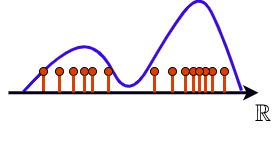
\includegraphics[width=0.35\textwidth]{Images/Quantile.png}
\vspace{-1.4cm}
\end{wrapfigure}

Оказывается, карты сложатся, если мы выберем другую аппроксимацию распределений в $\Prob (\R)$. Если раньше мы зафиксировали домен (узлы сетки) и подбирали вероятности, то теперь мы зафиксируем вероятности и будем подбирать узлы сетки. На первый взгляд это может показаться странно (как можно отказываться от предсказания вероятностей?), однако на самом деле это весьма гибкое семейство распределений с интересными свойствами. Итак:

\begin{definition}
Обозначим \emph{семейство квантильных распределений} $\mathcal{Q} \subset \Prob(\R)$ с $A$ атомами как множество равномерных дискретных распределений с $A$ произвольными исходами: если $\Z^*(s, a) \in \mathcal{Q}$, то для некоторых $A$ чисел $z_0, z_1 \dots z_{A-1} \colon$
$$\Prob \left( \Z^*(s, a) = z_i \right) = \frac{1}{A}$$
\end{definition}

Сразу хорошо то, что нам понадобится всего один гиперпараметр --- число атомов $A$ --- и не понадобится подбирать верхнюю-нижнюю границу ручками. Также заметим, что вырожденное распределение принадлежит $\mathcal{Q}$: просто все $z_i$ в этом случае совпадают.

$\B^*_D \Z^*_{\theta^-}$, тем не менее, может снова выпадать из такого семейства представлений, и нам всё равно понадобится какая-то проекция. Но на этот раз мы сможем сделать куда более естественную проекцию. На очередном шаге для заданной пары $s, a$ мы будем оптимизировать расстояние Вассерштайна $\W_1$ между правой частью уравнения Беллмана и тем, что мы выдаём:
\begin{equation}\label{qprojection}
\W_1 ([\B^*_D \Z^*_{\theta^-}](s, a) \parallel \Z) \to \min_{\Z \in \mathcal{Q}}
\end{equation}

Если бы умели выдавать произвольные распределения, мы бы искали $\Z$, условно, среди всех распределений и тогда выдали бы $[\B^*_D \Z^*_{\theta^-}](s, a)$, получив точный шаг метода простой итерации. Но поскольку мы ограничены семейством квантильных распределений, то лучшее, что мы можем сделать, это спроецировать шаг метода простой итерации в него. 

Ключевой момент: оказывается, задача \eqref{qprojection} имеет аналитическое решение. Введём следующее обозначение (<<середины отрезков сетки>>):
$$\tau_i \coloneqq \frac{\frac{i}{A} + \frac{i + 1}{A}}{2}$$

\begin{theorem}
Пусть $F$ --- функция распределения $[\B^*_D \Z^*_{\theta^-}](s, a)$. Тогда решение $\Z \in \mathcal{Q}$ задачи \eqref{qprojection} имеет домен $z_0, z_1 \dots z_{A-1}$:
$$z_i = F^{-1}(\tau_i)$$
\begin{proof}
Задача минимизации выглядит так:
\begin{equation}\label{Wassersteinminimization}
\int_0^1 \left| F^{-1}(\omega) - U^{-1}_{z_0, z_1 \dots z_{A-1}}(\omega) \right| \diff \omega \to \min_{z_0, z_1 \dots z_{A-1}}
\end{equation}
где $ U^{-1}_{z_0, z_1 \dots z_{A-1}}$ --- функция распределения равномерного дискретного распределения на домене $\{z_0, z_1 \dots z_{A-1}\}$. Чему она равна? Ну, понятно, что это такая <<лесенка>>:

\needspace{14\baselineskip}
\begin{wrapfigure}{r}{0.4\textwidth}
\vspace{-0.4cm}
\centering
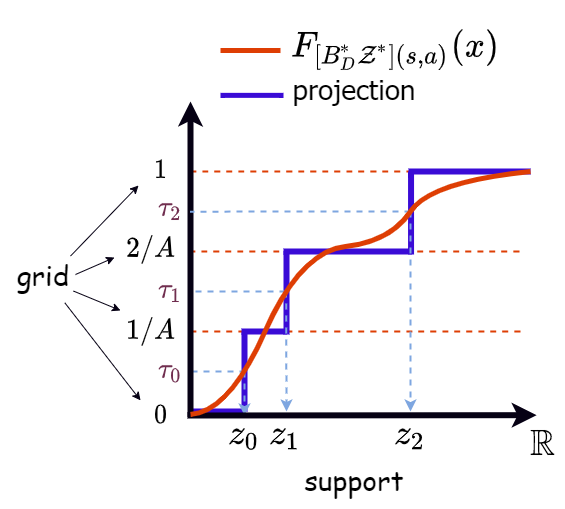
\includegraphics[width=0.4\textwidth]{Images/quantileprojection.png}
\vspace{-1.8cm}
\end{wrapfigure}

$$U^{-1}_{z_0, z_1 \dots z_{A-1}}(\omega) = \begin{cases}
z_0 \quad &0 \le \omega < \frac{1}{A} \\
z_1 \quad &\frac{1}{A} \le \omega < \frac{2}{A} \\
\vdots \\
z_{A - 1} \quad &\frac{A - 1}{A} \le \omega < 1
\end{cases}$$

Подставляем это в \eqref{Wassersteinminimization}:
\begin{equation*}
\sum_{i = 0}^{A - 1} \int_{\frac{i}{A}}^{\frac{i + 1}{A}} \left| F^{-1}(\omega) - z_i \right| d\omega \to \min_{z_0, z_1 \dots z_{A-1}}
\end{equation*}

Видим, что задача распадается на $A$ отдельных задач оптимизации:
\begin{equation}\label{w1minim}
\int_{\frac{i}{A}}^{\frac{i + 1}{A}} \left| F^{-1}(\omega) - z_i \right| d\omega \to \min_{z_i}
\end{equation}

Продифференцируем по $z_i$ и приравняем к нулю. Функция $F$ монотонна, поэтому сначала будет кусок интеграла, где градиент равен -1, затем кусок, где +1:
\begin{equation*}
\int_{\frac{i}{A}}^{F(z_i)} -1 \diff \omega + \int_{F(z_i)}^{\frac{i+1}{A}} 1 \diff \omega = 0
\end{equation*}
Берём интегралы от константы:
\begin{equation*}
-\left( F(z_i) - \frac{i}{A} \right) + \frac{i+1}{A} - F(z_i) = 0
\end{equation*}
Откуда видим $F(z_i) = \tau_i$ и получаем доказываемое.
\end{proof}
\end{theorem}

% Categorical DQN discovered a gap between theory and practice as $\KL$-divergence, used in practical algorithm, is theoretically unjustified. theorem \ref{DistributionalPolicyEvaluationConvergence} hints that the true divergence we should care about is actually Wasserstein metric, but it remained unclear how it could be optimized using only samples from transition probabilities $\Trans$.

% In \citep{dabney2018distributional} it was discovered that selecting another family of distributions to approximate $Z^*_\theta(s, a)$ will reduce Wasserstein minimization task to the search for quantiles of specific distributions. The latter can be done in online setting using \emph{quantile regression} technique. This led to alternative distributional Q-learning algorithm named Quantile Regression DQN (QR-DQN).

% The basic idea is to <<swap>> fixed support and learned probabilities of Categorical DQN. We will now consider the family with fixed probabilities for $A$-atomed categorical distribution with arbitrary support $\{ \zeta^*_0(s, a, \theta), \zeta^*_1(s, a, \theta), \dots , \zeta^*_{A - 1}(s, a, \theta)\}$. Again, we will assume all probabilities to be equal given the absence of any prior knowledge; namely, our distribution family is now
% $$Z^*_\theta(s, a) \sim \operatorname{Uniform}\left( \zeta^*_0(s, a, \theta), \dots , \zeta^*_{A - 1}(s, a, \theta) \right)$$
% In this setting neural network outputs $A$ arbitrary real numbers that represent the support of uniform categorical distribution\footnote{Note that target distribution is now guaranteed to remain within this distribution family as multiplying on $\gamma$ just shrinks the support and adding $r'$ just shifts it. We assume that if some atoms of the support coincide, the distribution is still $A$-atomed categorical; for example, for degenerated distribution (like in the case of terminal states) $\zeta^*_0(s, a, \theta) = \zeta^*_1(s, a, \theta) = \dots = \zeta^*_{A - 1}(s, a, \theta)$. This shows that projection step heuristic is not needed for this particular choice of distribution family.}, where $A$ is the number of atoms and the only hyperparameter to select.

% For table-case setting, on each step of point iteration we desire to update the cell for given state-action pair $s, a$ with full distribution of random variable to the right side of (\ref{optdistributionalBellman}). If we are limited to store only $A$ atoms of the support, the true distribution must be projected on the space of $A$-atomed categorical distributions. Consider now this task of projecting some given random variable with c.d.f. $F(\omega)$ in terms of Wasserstein distance. Specifically, we will be interested in minimizing $\mathcal{W}_1$-distance for $p = 1$ as the theorem \ref{DistributionalPolicyEvaluationConvergence} states the contraction property for all $1 \le p \le +\infty$ and we are free to choose any:



%\footnote{It can be proved that for table-case policy evaluation algorithm which stores in each cell not expectations of reward (as in Q-learning) but $A$ quantiles updated according to distributional Bellman equation (\ref{distributionalBellman}) using theorem \ref{quantilesisdesire} converges to quantiles of $Z^*(s, a)$ in Wasserstein metric for $1 \le p \le +\infty$ and its update operator is a contraction mapping in $\mathcal{W}_{\infty}$.}

\subsection{Quantile Regression DQN}\label{subsec:qrdqn}

\needspace{7\baselineskip}
\begin{wrapfigure}{r}{0.2\textwidth}
\vspace{-0.5cm}
\centering
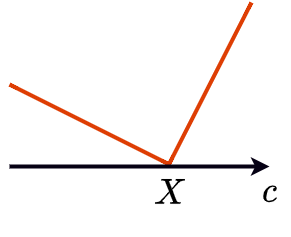
\includegraphics[width=0.2\textwidth]{Images/quantileloss.png}
\vspace{-1.2cm}
\end{wrapfigure}

Мы получили, что нам достаточно уметь искать лишь $A$ определённых квантилей распределения $\left[ \B^*_D \Z^* \right](s, a)$ для вычисления аппроксимации правой части уравнения Беллмана. Можем ли мы это сделать, используя только сэмплы? Конечно. 

\emph{Квантильная регрессия} (quantile regression) --- способ получить $\tau$-ый квантиль некоторого распределения, из которого доступна только лишь выборка. В частном случае, мы получим известный факт о том, что для получения медианы ($\frac{1}{2}$-го квантиля) нужно минимизировать MAE между константным прогнозом и сэмплами из распределения.

\begin{definition}
Для заданного $\tau \in (0, 1)$ \emph{квантильной функцией потерь} (quantile loss) называется:
\begin{equation}\label{quantileloss}
\Loss_{\tau}(c, X) \coloneqq \begin{cases}
\tau (c - X) \quad &c \ge X \\
(1 - \tau) (X - c) \quad &c < X \\
\end{cases}
\end{equation}
\end{definition}

\begin{theorem}[Квантильная регрессия] Решением задачи
\begin{equation}\label{QR}
\E_X \Loss_{\tau}(c, X) \to \min_{c \in \R}
\end{equation}
будет $\tau$-ый квантиль распределения случайной величины $X$.

\beginproof
Пусть $F$ --- функция распределения $X$. Распишем \eqref{QR}: для заданной точки $c$ интеграл будет состоять из двух слагаемых, где в первом $c < X$, а во втором $c \ge X$:
\begin{equation*}
\int_0^{F^{-1}(c)} (1 - \tau)(X - c) \diff \omega + \int_{F^{-1}(c)}^1 \tau (c - X) \diff \omega = 0 
\end{equation*}
Дифференцируем по $c$ и приравниваем к нулю:
\begin{equation*}
\int_0^{F^{-1}(c)} (\tau - 1) \diff \omega + \int_{F^{-1}(c)}^1 \tau \diff \omega = 0 
\end{equation*}
Берём константные интегралы:
\begin{equation*}
F^{-1}(c)(\tau - 1) + (1 - F^{-1}(c)) \tau = -F^{-1}(c) + \tau = 0
\end{equation*}
Отсюда получаем, что $F^{-1}(c) = \tau$, то есть $c$ --- $\tau$-ый квантиль. \qed
\end{theorem}

\begin{proposition}
Формулу \eqref{quantileloss} можно переписать <<в одну строчку>> в следующем виде:
$$\Loss_{\tau}(c, X) = \left( \tau - \mathbb{I}[c < X] \right) \left( c - X \right)$$
\end{proposition}

\needspace{7\baselineskip}
\begin{wrapfigure}{r}{0.2\textwidth}
%\vspace{-0.5cm}
\centering
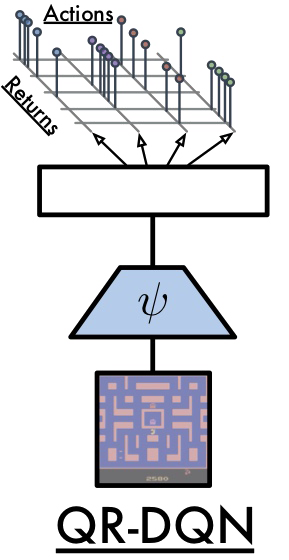
\includegraphics[width=0.2\textwidth]{Images/qrdqn.png}
\vspace{-0.5cm}
\end{wrapfigure}
Итак, соберём всё вместе. У нас есть нейросеть $z_i(s, a, \theta)$ с параметрами $\theta$, которая для данного состояния-действия выплёвывает $A$ произвольных вещественных чисел, которые мы интерпретируем как $A$ равновероятных возможных исходов случайной величины $\Z^*(s, a, \theta)$. Обозначим за $\theta^-$ веса таргет-сети, как обычно. Для очередного перехода $\T \coloneqq (s, a, r, s', \done)$ из буфера мы хотим провести оптимизацию
\begin{equation}\label{wassersteinminim}
\W_1(\left[\B^*_D \Z^*\right](s, a, \theta^{-}) \parallel \Z^*(s, a, \theta)) \to \min_\theta
\end{equation}
и мы поняли, что это эквивалентно поиску квантилей распределения $\left[\B^*_D \Z^*\right](s, a, \theta^{-})$, поэтому для оптимизации $i$-го выхода нейросетки будем оптимизировать квантильный лосс \eqref{quantileloss} (по $i$ просто просуммируем --- хотим учить все $A$ интересующих нас квантилей):
$$\sum_{i=0}^{A-1} \E_{x \sim \left[\B^*_D \Z^*\right](s, a, \theta^{-})} \Loss_{\tau_i}(z_i(s, a, \theta), x) \to \min_{\theta}$$

Конечно же, мы не будем доводить этот процесс оптимизации до конца, а сделаем всего один шаг обновления весов $\theta$ по градиенту, а затем сразу же возьмём из буфера другой мини-батч. Мы лишь получили способ получать несмещённые оценки градиентов, указывающих в сторону минимизации \eqref{wassersteinminim}.

Опять же заметим, что $\E_{x \sim \left[\B^*_D \Z^*\right](s, a, \theta^{-})}$ распадается в сэмплирование $s'$ и интегрирование по возможным исходам $\Z^*(s', \pi^*(s'))$, где $\pi^*(s')$ выбирает действие жадно. Мат.ожидание по $\Z^*(s', a', \theta^{-})$ при данных $s', a'$ есть просто усреднение по $A$ равновероятным исходам, поэтому его мы посчитаем явно. Итого:
$$\underbrace{\sum_{i=0}^{A-1}}_{\mathclap{\text{\shortstack{учим $A$ \\ квантилей}}}} \overbrace{\E_{s'} \frac{1}{A}}^{\mathclap{\text{\shortstack{вероятности \\ сэмплов}}}}\sum_{j=0}^{A-1} \Loss_{\tau_i}(\underbrace{z_i(s, a, \theta)}_{\text{прогноз}}, \overbrace{r + \gamma z_j(s', a', \theta^{-})}^{\text{сэмпл}}) \to \min_{\theta}$$
Занося внешнюю сумму под мат.ожидание по $s'$, получаем функцию потерь, градиент которой можно оценивать по Монте-Карло, используя лишь сэмплы $s'$ из функции переходов.

\begin{algorithm}[label = QRDQNalgorithm]{Quantile Regression DQN (QR-DQN)}
\textbf{Гиперпараметры:} $B$ --- размер мини-батчей, $A$ --- число атомов, $K$ --- периодичность обновления таргет-сети, $\eps(t)$ --- стратегия исследования, $z_i(s, a, \theta)$ --- нейросетка с параметрами $\theta$, SGD-оптимизатор

\vspace{0.3cm}
Предпосчитать середины отрезков квантильной сетки $\tau_i \coloneqq \frac{\frac{i}{A} + \frac{i+1}{A}}{2}$ \\
Инициализировать $\theta$ произвольно \\
Положить $\theta^- \coloneqq \theta$ \\
Пронаблюдать $s_0$ \\
\textbf{На очередном шаге $t$:}
\begin{enumerate}
    \item выбрать $a_t$ случайно с вероятностью $\eps(t)$, иначе $a_t \coloneqq \argmax\limits_{a_t} \sum_{i=0}^{A-1} z_i(s_t, a_t, \theta)$
    \item пронаблюдать $r_t$,  $s_{t+1}$, $\done_{t+1}$
    \item добавить пятёрку $(s_t, a_t, r_t, s_{t+1}, \done_{t+1})$ в реплей буфер
    \item засэмплировать мини-батч размера $B$ из буфера
    \item для каждого перехода $\T \coloneqq (s, a, r, s', \done)$ посчитать таргет:
    $$y(\T)_j \coloneqq r + (1 - \done)\gamma z_j\left( s', \argmax\limits_{a'} \sum_{i} z_i(s', a', \theta^-), \theta^- \right) $$
    \item посчитать лосс:
    $$\Loss(\theta) \coloneqq \frac{1}{BA}\sum_{\T} \sum_{i=0}^{A-1} \sum_{j=0}^{A-1} \left( \tau_i - \mathbb{I}[z_i(s, a, \theta) < y(\T)_j] \right) \left( z_i(s, a, \theta) - y(\T)_j \right)$$
    \item делаем шаг градиентного спуска по $\theta$, используя $\nabla_\theta \Loss(\theta)$
    \item если $t \operatorname{mod} K = 0$: $\theta^- \gets \theta$
\end{enumerate}
\end{algorithm}

\subsection{Implicit Quantile Networks}\label{subsec:iqn}

В QR-DQN мы фиксировали <<равномерную сетку>> на оси квантилей: говорили, что наше аппроксимирующее распределение есть равномерное на домене из $A$ атомов. Идея: давайте будем уметь в нашей нейросети выдавать произвольные квантили, каким-то образом задавая $\tau \in (0, 1)$ дополнительно на вход. Тогда наша модель $z(s, a, \tau, \theta)$ будет неявно (implicit) задавать, вообще говоря, произвольное распределение на $\R$. По сути, мы моделируем квантильную функцию <<целиком>>; очень удобно:
$$F^{-1}_{\Z^*(s, a)}(\tau) \coloneqq z(s, a, \tau, \theta)$$

Поймём, как тогда считать мат.ожидание (или Q-функцию) в такой модели.

\begin{theoremBox}[label=th:samplingimplicit]{}
Пусть $F$ --- функция распределения случайной величины $X$. Тогда, если $\tau \sim U[0, 1]$, случайная величина $F^{-1}(\tau)$ имеет то же распределение, что и $X$.
\beginproof
Заметим, что функция распределения равномерной случайной величины при $x \HM\in [0, 1]$ равна $\Prob(\tau \HM< x) \HM= x$. Теперь посмотрим на функцию распределения случайной величины $F^{-1}(\tau)$:
\begin{equation*}
\Prob \left( F^{-1}(\tau) < x \right) = \Prob \left( \tau < F(x) \right) = F(x) \tagqed   
\end{equation*}
\end{theoremBox}

\needspace{7\baselineskip}
\begin{wrapfigure}{r}{0.25\textwidth}
\vspace{-0.3cm}
\centering
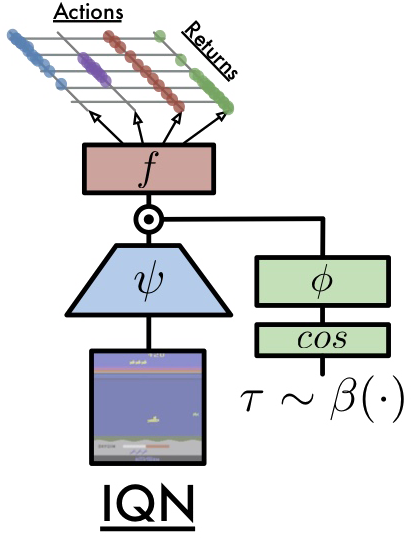
\includegraphics[width=0.25\textwidth]{Images/iqn.png}
\vspace{-1.5cm}
\end{wrapfigure}

Итак, мы можем аппроксимировать жадную стратегию примерно так:
$$\pi^*(s) = \argmax\limits_{a} \sum_{i=0}^{N} z(s, a, \tau_i, \theta), \qquad \tau_i \sim U[0, 1]$$

В качестве функции потерь предлагается использовать тот же квантильный лосс, что и в QR-DQN, только если в QR-DQN нам были нужны определённые $A$ квантилей, то теперь предлагается засэмплировать $N'$ каких-то квантилей и посчитать лосс для них. Для подсчёта лосса нам было нужно брать мат.ожидание по $\Z^*_{\theta^-}(s', a')$, для чего в формуле мы пользовались тем, что это распределение в нашей модели равномерно. Теперь же этот интеграл мы заменяем на Монте-Карло оценку с произвольным числом сэмплов $N''$, а для сэмплирования опять же используем теорему \ref{th:samplingimplicit}:
$$\Loss(\T, \theta) \coloneqq \sum_{i=0}^{N'} \frac{1}{N''} \sum_{j=0}^{N''} \Loss_{\tau_i}(z(s, a, \tau_i, \theta), r + \gamma z(s', \pi^*(s'), \tau_j, \theta^{-})),$$
где $\tau_i, \tau_j \sim U[0, 1]$.

\begin{remark}
Архитектура сети предлагается такая. Входное состояние сжимается в некоторый эмбеддинг при помощи основной части сети $f(s, \theta)$. Параллельно строится некоторый эмбеддинг $g(\tau, \theta)$, описывающий квантиль $\tau \in (0, 1)$: тут могут быть разные варианты, но авторы остановились на следующем: число $\tau$ <<описывается>> несколькими признаками, где $i$-ый признак равен $\cos(\pi i \tau)$, и преобразуется одним полносвязным слоем (с обучаемыми параметрами) для получения $g(\tau, \theta)$. Дальше финальное преобразование $h$ должно взять $f(s, \theta)$ и $g(\tau, \theta)$ и выдать по одному числу для каждого действия $a$; чтобы не городить ещё слои, взаимодействие этих двух эмбеддингов предлагается организовать при помощи поэлементного перемножения:
$$z(s, a, \tau, \theta) \coloneqq h(f(s, \theta) \odot g(\tau, \theta), \theta)$$
\end{remark}

\subsection{Rainbow DQN}\label{subsec:rainbow}

В разделе про модификации \ref{sec:dqnmods} были рассмотрены весьма разные улучшения DQN, нацеленные на решения очень разных проблем. Хорошо видно, что все эти модификации <<ортогональны>> и могут включаться-выключаться, так сказать, независимо в алгоритм. Distributional-подход, вообще говоря, не решает какую-то проблему внутри DQN, но может рассматриваться как ещё одна модификация базового алгоритма DQN.

Rainbow DQN совмещает 6 модификаций алгоритма DQN:
\begin{itemize}
    \item Double DQN (раздел \ref{subsec:doubledqn})
    \item Dueling DQN (раздел \ref{subsec:duelingdqn})
    \item Noisy DQN  (раздел \ref{subsec:noisynets})
    \item Prioritized Experience Replay (раздел \ref{subsec:prioritizedreplay})
    \item Multi-step DQN (раздел \ref{subsec:multistepdqn})
    \item Distributional RL
\end{itemize}

В последнем пункте исторически в Rainbow используется Categorical DQN (раздел \ref{subsec:c51}), однако понятно, что можно использовать любой другой алгоритм; в частности, QR-DQN (раздел \ref{subsec:qrdqn}) или IQN (раздел \ref{subsec:iqn}). Обсудим только пару нюансов, которые возникают при совмещении некоторых пар из этих идей, а дальше приведём полный-полный алгоритм.

Совмещение приоритизированного реплея и Distributional-подхода требует введения приоритета перехода $\T$: в его качестве, аналогично обычному случаю \eqref{priority}, берётся значение функции потерь \eqref{c51loss}: 
$$\rho(\T) \coloneqq \KL(y(\T) \parallel \Z^*(s, a, \theta))$$

При совмещении шумных сетей с эвристикой Double DQN, шум сэмплируется заново на каждом проходе через сеть или таргет-сеть (то есть генерится отдельный сэмпл шума для выбора действия $a'$, отдельный для оценивания при построении таргета и отдельный для прохода через сеть для подсчёта градиентов).

Забивать костыльми приходится совмещение Categorical DQN с Dueling DQN. Здесь остаётся только идея о том, что при обновлении модели для пары $s, a$ мы должны <<легче обобщаться>> на все остальные действия $\hat{a} \in \A$, для чего вычисление $p_i(s, a, \theta)$ проходит в два потока: <<типа>> V-поток $V(s, \theta)$, который выдаёт $A$ атомов как бы общих для всех действий, и <<типа>> A-поток $A(s, a, \theta)$, который выдаёт $A$ атомов для каждого из $|\A|$ действий. Дальнейшая формула <<взята>> из обычного Dueling DQN \eqref{dueling}; софтмакс, необходимый, чтобы получить на выходе валидное категориальное распределение, применяется в самом конце:
\begin{equation}\label{rainbowdueling}
p_i(s, a, \theta) \coloneqq \softmax\limits_{i} \left( V(s, \theta)_i + A(s, a, \theta)_i - \frac{1}{|\A|}\sum_a A(s, a, \theta)_i \right)
\end{equation}
Последнее слагаемое --- <<типа>> централизация A-потока к нулю, снова со средним вместо максимума (хотя эта логика к вероятностям исходов $\Z^*$ уже плохо применима).

\begin{remark}
Ablation study там показывал, что убирание Dueling DQN, в отличие от остальных 5 модификаций, к особому падению качества итогового алгоритма не приводит. Вероятно, это связано с тем, что <<семантика>> потоков ещё больше теряется.
\end{remark}

\begin{algorithm}[label = rainbowalg]{Rainbow DQN}
\textbf{Гиперпараметры:} $B$ --- размер мини-батчей, $V_{\max}, V_{\min}, A$ --- параметры категориальной аппроксимации, $K$ --- периодичность обновления таргет-сети, $N$ --- количество шагов в оценке, $\alpha$ --- степень приоритизации, $\beta(t)$ --- параметр importance sampling коррекции для приоритизированного реплея, $p_i(s, a, \theta, \eps)$ --- нейросетка с параметрами $\theta$, SGD-оптимизатор

\vspace{0.3cm}
Предпосчитать узлы сетки $z_i \coloneqq V_{\min} + \frac{i}{A}(V_{\max} - V_{\min})$ \\
Инициализировать $\theta$ произвольно \\
Положить $\theta^- \coloneqq \theta$ \\
Пронаблюдать $s_0$ \\
\textbf{На очередном шаге $t$:}
\begin{enumerate}
    \item выбрать $a_t \coloneqq \argmax\limits_{a_t} \sum_{i=0}^A z_i p_i(s_t, a_t, \theta, \eps), \quad \eps \sim \N(0, I)$
    \item пронаблюдать $r_t$, $s_{t+1}$, $\done_{t+1}$
    \item построить $N$-шаговый переход $\T \coloneqq \left( s, a, \sum_{n=0}^N \gamma^n r^{(n)}, s^{(N)}, \done \right)$, используя последние $N$ наблюдений, и добавить его в реплей буфер с максимальным приоритетом %$\max\limits_{\T} \rho(\T)$
    \item засэмплировать мини-батч размера $B$ из буфера, используя вероятности $\Prob (\T) \propto \rho(\T)^\alpha$
    \item посчитать веса для каждого перехода:
    $$w(\T) \coloneqq \frac{1}{\rho(\T)^{\beta(t)}}$$
    \item для каждого перехода $\T \coloneqq (s, a, \bar{r}, \bar{s}, \done)$ посчитать таргет:
    $$\eps_1, \eps_2 \sim \N(0, I)$$
    $$\Prob \left( y(\T) = \bar{r} + \gamma^N z_i \right) \coloneqq p_i\left( \bar{s}, \argmax_{\bar{a}} \sum_{i=0}^A z_i p_i(\bar{s}, \bar{a}, \theta, \eps_1), \theta^-, \eps_2 \right)$$
    \item спроецировать таргет на сетку $\{ z_0, z_1 \dots z_{A} \}$: $y(\T) \leftarrow \Pi y(\T)$ 
    \item посчитать для каждого перехода лосс:
    $$L(\T, \theta) \coloneqq -\sum_{i=0}^{A} \Prob \left( y(\T) = z_i \right) p_i(s_t, a_t, \theta, \eps) \quad \eps \sim \N(0, I)$$
    \item обновить приоритеты всех переходов из буфера: $\rho(\T) \gets L(\T, \theta)$
    \item посчитать суммарный лосс:
    $$\Loss(\theta) \coloneqq \frac{1}{B}\sum_{\T} w(\T)L(\T, \theta)$$
    \item делаем шаг градиентного спуска по $\theta$, используя $\nabla_\theta \Loss(\theta)$
    \item если $t \operatorname{mod} K = 0$: $\theta^- \gets \theta$
\end{enumerate}
\end{algorithm}